%% =============================================================================
%% PRACTICE FINAL — assembled from the question bank.
%% Each question is a fragment; reorder / swap by editing the \input list.
%%
%% Assignment rationale is in final_status.md.
%% Deliberately covers the same topics as the real final with DIFFERENT problems.
%% =============================================================================

%% Retitles the cover page and running header to "Practice Final".
\def\practiceversion{}
%% Solutions are ON unless \blankversion is defined before this file is read.
%% The Makefile builds the blank version with:
%%     pdflatex "\def\blankversion{}%% =============================================================================
%% REAL FINAL -- all questions inlined.
%%
%% Previously this file was an \input list over q/*.tex and draft_*.tex; the
%% question bodies now live here directly, in exam order. q/preamble.tex is
%% still \input, since it is shared with exam_practice.tex (it carries the
%% documentclass, the cover page, and the \blankversion / \practiceversion
%% switches).
%%
%% NOTE: the CPS slot is Binary Decision Trees (30 pts). Its 12-pt `compress`
%%       part is staged -- students get the if/else-if/else skeleton with the
%%       conditions filled in. "Filling in the Blanks" is the lighter
%%       alternative, on the practice exam.
%% =============================================================================

%% Solutions are ON unless \blankversion is defined before this file is read.
%% The Makefile builds the blank version with:
%%     pdflatex "\def\blankversion{}\input{exam_final.tex}"
\ifdefined\blankversion
  \documentclass[addpoints,12pt]{exam}
\else
  \documentclass[addpoints,12pt,answers]{exam}
\fi

%% exam_practice.tex sets \practiceversion before reading this file; that
%% swaps every "Final Exam" below over to "Practice Final".
\ifdefined\practiceversion
  \newcommand{\examname}{Practice Final}
  \newcommand{\drawprompt}{Feel free to use this space to draw Polly the Polymorphic Parrot, the class mascot!}
  \newcommand{\drawboxheight}{1.9in}
\else
  \newcommand{\examname}{Final Exam}
  \newcommand{\drawprompt}{Feel free to use this space to draw \textbf{anything you like}. You're free!}
  \newcommand{\drawboxheight}{3.5in}
\fi

\usepackage{amsmath, amsthm, amssymb, amsfonts}
\usepackage{thmtools}
\usepackage{graphicx}
\usepackage[hidelinks]{hyperref}
\usepackage[utf8]{inputenc}
\usepackage[english]{babel}
\usepackage{framed}
\usepackage[dvipsnames]{xcolor}
\usepackage{tcolorbox}
\usepackage{tabto}
\usepackage{titling}
\usepackage{tikz}
\usepackage{dirtree}

\usetikzlibrary{patterns}
\tikzset{
level distance=13mm,
every child/.style={line width=0.3mm},
black/.style={text=white, circle, draw=black, line width=0.4mm, inner sep=4pt},
red/.style={text=white, circle, draw=black, line width=0.4mm, inner sep=4pt},
unknown/.style={text=white, circle, draw=black, line width=0.4mm, inner sep=4pt, preaction={fill, pink!90!black}, pattern=north east lines,distance=0.5pt},
}

\usepackage{changepage} % for the adjustwidth environment


\colorlet{LightGray}{White!90!Periwinkle}
\colorlet{LightOrange}{Orange!15}
\colorlet{LightGreen}{Green!15}

\newcommand{\HRule}[1]{\rule{\linewidth}{#1}}

\declaretheoremstyle[name=Theorem,]{thmsty}
\declaretheorem[style=thmsty,numberwithin=section]{theorem}
\tcolorboxenvironment{theorem}{colback=LightGray}

\declaretheoremstyle[name=Proposition,]{prosty}
\declaretheorem[style=prosty,numberlike=theorem]{proposition}
\tcolorboxenvironment{proposition}{colback=LightOrange}

\declaretheoremstyle[name=Principle,]{prcpsty}
\declaretheorem[style=prcpsty,numberlike=theorem]{principle}
\tcolorboxenvironment{principle}{colback=LightGreen}

%% This latex package provides all the utilities for
%% 15150 assignments development.
%% This package is intended to be included in writeup.tex at
%% problem level.
%% For a full list of custom commands, check 15150toolbox.md
%%
%% @author: Jolin Zhou
%% @email: jiulingz@andrew.cmu.edu

\NeedsTeXFormat{LaTeX2e}
\ProvidesPackage{toolbox-reduced}[2020/05/15 Latex toolbox for M20 Lecture Notes]

%%%%%%%%%%%%%%%%%%%%%
%% Robust Commands %%
%%%%%%%%%%%%%%%%%%%%%
% used throughout this package
\RequirePackage{etoolbox}
\RequirePackage{xparse}

% hyperlink/reference
\RequirePackage{xcolor}

% graphics
\RequirePackage{graphicx}

% emphasize
\usepackage{bm}
\DeclareTextFontCommand{\emph}{\bfseries\em}

%%%%%%%%%%%%%%%%%%%%%%%%%%%%%%%
%% Task related environments %%
%%%%%%%%%%%%%%%%%%%%%%%%%%%%%%%
% environment colors
\RequirePackage{xcolor}
\definecolor{task_color}      {RGB}{ 64, 100, 255}
\definecolor{solution_color}  {RGB}{  0,   0, 128}
\definecolor{constraint_color}{RGB}{175,   0,   0}

% task environment
\RequirePackage{framed}
\providerobustcmd{\attribute}[1]{}
\newcounter{taskcounter}
\NewDocumentEnvironment{task}{m}
{
  \stepcounter{taskcounter}
  \textbf{Task \arabic{taskcounter}.}\attribute{#1}
  \phantomsection
  \addcontentsline{toc}{subsubsection}{\textcolor{task_color}{\textbf{Task \arabic{taskcounter}.}\texorpdfstring{\attribute{#1}}{}}}
  \par
}
{
  \ifdef{\loadsolution}
    {{
      \color{solution_color}
      \begin{framed}
        \textbf{Solution \arabic{taskcounter}.}\par
        \loadsolution{#1}
      \end{framed}
    }}
    {}
  \vspace{1em}
}

% constraint environment
\newenvironment{constraint}{\color{constraint_color}\textbf{Constraint:}}{}

%%%%%%%%%%%%%%%%%%%%%%%%
%% Code Specification %%
%%%%%%%%%%%%%%%%%%%%%%%%
% spec
\RequirePackage{framed}
\usepackage{mdframed}
\newrobustcmd{\spec}[4]{
\begin{mdframed}
\code{#1 :} #2\par
\ifstrempty{#3}{}{\par REQUIRES: #3}
\ifstrempty{#4}{}{\par ENSURES: #4}
\end{mdframed}
}

%%%%%%%%%%%%%%%%%%%%%
%% Text Formatting %%
%%%%%%%%%%%%%%%%%%%%%
% symbols
\RequirePackage{amssymb, amsmath, amsthm, amsfonts}

\newrobustcmd{\stepsTo}{\Longrightarrow}
\newrobustcmd{\stepsToStar}{\Longrightarrow}
\newrobustcmd{\stepsToIn}[1]{\Longrightarrow^{#1}}

\newrobustcmd{\eeq}{\cong}

%%%%%%%%%%%%%%%%%%%%%%
%% Code Environment %%
%%%%%%%%%%%%%%%%%%%%%%
% code style
\RequirePackage{listings}
\RequirePackage{lstautogobble}
\RequirePackage{xcolor}

\newlength{\MaxSizeOfLineNumbers}%
\settowidth{\MaxSizeOfLineNumbers}{99}% Adjust to maximum number of lines
\addtolength{\MaxSizeOfLineNumbers}{.5ex}%

\newcommand{\darkBg}{8b98ad}
\definecolor{background_color}{RGB}{225, 225, 225}
\definecolor{string_color}    {RGB}{180, 156,   0}
\definecolor{keyword_color}   {RGB}{ 64, 100, 255}
\definecolor{comment_color}   {RGB}{  140, 140, 140}
\definecolor{number_color}    {RGB}{ 84,  84,  84}
\lstdefinestyle{15150code}{
    basicstyle=\ttfamily,
    numberstyle=\tiny\ttfamily\color{number_color},
    stringstyle=\color{string_color},
    keywordstyle=\color{blue!90!black},
    commentstyle=\color{comment_color},
    numbers=left,
    rulesepcolor=\color{black!20!white},
    linewidth=\textwidth,
    columns=fixed,
    tabsize=2,
    xleftmargin=\MaxSizeOfLineNumbers,
    breaklines=true,
    keepspaces=true,
    showstringspaces=false,
    captionpos=b,
    autogobble=true,
    mathescape=true,
    literate={~}{{$\thicksim$}}1
             {~=}{{$\eeq$}}1
}
\lstdefinelanguage{sml}{
    language=ML,
    morestring=[b]",
    morecomment=[s]{(*}{*)},
    morekeywords={
        bool, char, exn, int, real, string, unit, list, option,
        EQUAL, GREATER, LESS, NONE, SOME, nil,
        andalso, orelse, true, false, not,
        if, then, else, case, of, as,
        let, in, end, local, val, rec,
        datatype, type, exception, handle,
        fun, fn, op, raise, ref,
        structure, struct, signature, sig, functor,
        include, open, use, infix, infixr, o, print
    }
}

\usepackage[T1]{fontenc}

\makeatletter
\newenvironment{btHighlight}[1][]
{\begingroup\tikzset{bt@Highlight@par/.style={#1}}\begin{lrbox}{\@tempboxa}}
{\end{lrbox}\bt@HL@box[bt@Highlight@par]{\@tempboxa}\endgroup}

\newcommand\btHL[1][]{%
  \begin{btHighlight}[#1]\bgroup\aftergroup\bt@HL@endenv%
}
\def\bt@HL@endenv{%
  \end{btHighlight}%
  \egroup
}
\newcommand{\bt@HL@box}[2][]{%
  \tikz[#1]{%
    \pgfpathrectangle{\pgfpoint{1pt}{0pt}}{\pgfpoint{\wd #2}{\ht #2}}%
    \pgfusepath{use as bounding box}%
    \node[anchor=base west, fill=yellow!45,outer sep=0pt,inner xsep=1pt, inner ysep=0pt, rounded corners=3pt, minimum height=\ht\strutbox+1pt,#1]{\raisebox{1pt}{\strut}\strut\usebox{#2}};
  }%
}

\newenvironment{atHighlight}[1][]
{\begingroup\tikzset{at@Highlight@par/.style={#1}}\begin{lrbox}{\@tempboxa}}
{\end{lrbox}\at@HL@box[at@Highlight@par]{\@tempboxa}\endgroup}

\newcommand\atHL[1][]{%
  \begin{atHighlight}[#1]\bgroup\aftergroup\at@HL@endenv%
}
\def\at@HL@endenv{%
  \end{atHighlight}%
  \egroup
}
\newcommand{\at@HL@box}[2][]{%
  \tikz[#1]{%
    \pgfpathrectangle{\pgfpoint{1pt}{0pt}}{\pgfpoint{\wd #2}{\ht #2}}%
    \pgfusepath{use as bounding box}%
    \node[anchor=base west, fill=red!45,outer sep=0pt,inner xsep=1pt, inner ysep=0pt, rounded corners=3pt, minimum height=\ht\strutbox+1pt,#1]{\raisebox{1pt}{\strut}\strut\usebox{#2}};
  }%
}
\makeatother

% code inline
\newrobustcmd{\code}[2][]{{\sloppy
\ifmmode
    \text{\lstinline[language=sml,style=15150code,#1]`#2`}
\else
    {\lstinline[language=sml,style=15150code,#1]`#2`}%
\fi}}

% code block
\lstnewenvironment{codeblock}[1][]{\lstset{
  language=sml,
  style=15150code,numbers=none,#1,moredelim=**[is][\btHL]{`}{`},moredelim=**[is][\atHL]{&}{&}}}{}

% ------------------------------------------------------------------------------

\begin{document}

% Use the exam class's native headers/footers. (fancyhdr 1.11b conflicts
% with the exam class, which already defines \lhead/\rhead/\chead.)
\pagestyle{headandfoot}
\header{\examname}{}{15-150: Principles of Functional Programming}
\footer{}{\thepage}{}

% ------------------------------------------------------------------------------
% Cover Page and ToC
% ------------------------------------------------------------------------------

\setlength{\droptitle}{-8em}   % This is your set screw

\title{ \normalsize \textsc{}
		\HRule{1.5pt} \\
		\large \textbf{
      \uppercase{\examname} \\
      15-150 Principles of Functional Programming M26} \\
    \vspace{-0.15cm}
    \HRule{1.5pt}
}
\date{}

\maketitle

\vspace{-2.5cm}

Name \rule{6cm}{0.4pt} \, Andrew ID \rule{6cm}{0.4pt}

\vspace{20pt}

%% Left-aligned, and pulled slightly PAST the left margin. \noindent kills the
%% paragraph indent; the negative \hspace then moves the whole block into the
%% margin. The itemize's own \leftmargin is zeroed so the bullets themselves sit
%% at the block's edge rather than ~2.5em inside it. The old version wrapped both
%% minipages in a `center` and fought it with \hspace{-3cm}.
%% The \makebox is what keeps the negative shift from overflowing the line: it
%% pins the pair's advertised width to \textwidth and left-aligns the contents,
%% so the 0.8cm pull into the margin costs no horizontal budget.
\noindent\makebox[\textwidth][l]{%
\hspace*{-0.8cm}%
\begin{minipage}{0.585\textwidth}
\setlength{\leftmargini}{1.2em}
\begin{itemize}
  \item Write your name and Andrew ID on this page.
  \vspace{-5pt}
  \item This is a 180 minute examination of 8 parts.
  \vspace{-5pt}
  \item Answers should be short and to the point. Obey question constraints, wherever
  they appear, and write syntactically legal SML programs!
  \vspace{-5pt}
  \item At any point on this examination, you are allowed to use the \code{map},
  \code{filter}, \code{foldl}, \code{foldr}, \code{length}, \code{o}, and \code{@} functions,
  as seen in lecture.
  \vspace{-5pt}
  \item A box having lots of space does not imply the answer will be long or convoluted. If your
  answer is ugly, it's likely that something is wrong with your approach.
  \item I have full faith in you. You're going to do great.
\end{itemize}
\end{minipage}
\hspace{10pt}
\begin{minipage}{0.35\textwidth}
{\small
\vqword{}
\vpword{Max}
\begin{center}
\gradetable[v][questions]
\end{center}
}
\end{minipage}%
}

\vspace{\fill}

%% The drawing box is sized to whatever vertical room is left after the bullets
%% and the grade table. The practice exam's table has longer question titles, so
%% a fixed 2.5in box overflows and LaTeX silently drops the whole block --
%% \drawboxheight lets each version ask for a height that actually fits.
\begin{center}
  \drawprompt \\

  \vspace{8pt}

  \fbox{\rule{6in}{0pt}\rule[-0.5ex]{0pt}{\drawboxheight}}
\end{center}


\newpage

% ------------------------------------------------------------------------------

\section*{Questions}

\begin{questions}

%% --- openers -----------------------------------------------------------------
%% (was \titledquestion{Types and Values}
\textbf{Types and Values}

For each of the expressions below, write its \textbf{most general type} and value.

\textbf{If the expression is not well-typed then say so and explain your answer briefly.}

\textbf{If the expression does not evaluate to a value then say so and explain your answer briefly.}

\textbf{For brevity, if the expression is already a value, you may write out "same" for its value}.

\begin{parts}

  \part[2]\hfill

  In the context of the declaration
  \begin{codeblock}
    datatype ('a, 'b) pair = P of 'a * 'b
  \end{codeblock}
  consider:
  \begin{codeblock}
    fn x => P (x, [x])
  \end{codeblock}

  \textbf{Type:} \begin{solutionorlines}[2em] \code{'a -> ('a, 'a list) pair} \end{solutionorlines}

  \textbf{Value:} \begin{solutionorlines}[2em] same \end{solutionorlines}

  \vspace{10pt}

  \part[2]\hfill

  \begin{codeblock}
    fn f => filter (map f)
  \end{codeblock}

  \textbf{Type:} \begin{solutionorlines}[2em] NWT \end{solutionorlines}

  \textbf{Value:} \begin{solutionorlines}[2em] No value \end{solutionorlines}

  \vspace{10pt}

  \part[2]\hfill

  \begin{codeblock}
    let
      val r1 = ref 0
      val r2 = ref r1
      val () = r2 := ref (!r1)
      val () = r1 := 1
      val () = (!r2) := !!r2 + !!r2
    in
      !!r2 + !r1
    end
  \end{codeblock}

  \textbf{Type:} \begin{solutionorlines}[2em] \code{int} \end{solutionorlines}

  \textbf{Value:} \begin{solutionorlines}[2em] \code{1} \end{solutionorlines}

  \vspace{10pt}

  \part[2]\hfill

  \begin{codeblock}
    val x = 2
    fun foo y z = x + y + z
    val x = 3
    val res = x + foo x x
  \end{codeblock}

  What is the type and value of \code{res}?

  \textbf{Type:} \begin{solutionorlines}[2em] \code{int} \end{solutionorlines}

  \textbf{Value:} \begin{solutionorlines}[2em] \code{11} \end{solutionorlines}

  \part[2]\hfill

  \begin{codeblock}
    fn f => fn g => fn x => g (f x, x)
  \end{codeblock}

  \textbf{Type:} \begin{solutionorlines}[3em] \code{('a -> 'b) -> ('b * 'a -> 'c) -> 'a -> 'c} \end{solutionorlines}

  \textbf{Value:} \begin{solutionorlines}[2em] same \end{solutionorlines}
\end{parts}

\newpage
)
\titledquestion{Types and Values}
\textbf{Types and Values}

For each of the expressions below, write its \textbf{most general type} and value.

\textbf{If the expression is not well-typed then say so and explain your answer briefly.}

\textbf{If the expression does not evaluate to a value then say so and explain your answer briefly.}

For brevity, if the expression is already a value, you may write out "same" for its value.

If the value involves a recursive function body, you may write "<body>" instead.

\begin{parts}

  %% (was `fn x => P (x, [x])` over a two-parameter `('a, 'b) pair`, which leaned
  %%  on double polymorphism; then a version with `None` in the second field,
  %%  which turned on noticing `'a * 'a` rather than `'a bag * 'a bag` -- a
  %%  misread lost the whole part. Here both fields are visibly the same
  %%  expression, so nothing hinges on parsing the declaration: the work is
  %%  composing 'a -> 'a bag -> 'a bag bag.
  %%  Verified in SML/NJ: `int -> int bag bag` typechecks, `int -> int bag` is
  %%  rejected with a tycon mismatch.)
  \part[2]\hfill

  In the context of the declaration
  \begin{codeblock}
    datatype 'a bag = None | Two of 'a * 'a
  \end{codeblock}
  consider:
  \begin{codeblock}
    fn x => Two (Two (x, x), Two (x, x))
  \end{codeblock}

  \textbf{Type:} \begin{solutionorlines}[4em] \code{'a -> 'a bag bag} \\[2pt]
  Each inner \code{Two (x, x)} has type \code{'a bag}. The outer \code{Two} then
  holds two of \textit{those}, so its element type is \code{'a bag} and the
  result is \code{'a bag bag}. \end{solutionorlines}

  \textbf{Value:} \begin{solutionorlines}[2em] same \end{solutionorlines}

  \vspace{10pt}

  %% (was `fn f => filter (map f)`, an NWT one-liner; then `map o foldl`, which
  %%  was a puzzle rather than code anyone writes. This is the ordinary
  %%  "partially apply a curried function, then map the rest" idiom, and it still
  %%  tests both points: applying `f` to `x` CONSUMES f's first argument, and the
  %%  leftover `'b -> 'c` is what fixes map's element and result types.
  %%  Verified in SML/NJ -- no value restriction, both `fun` and `fn` forms give
  %%    ('a -> 'b -> 'c) -> 'a -> 'b list -> 'c list
  %%  and e.g. it applied to (fn a => fn b => a * b) and 3 maps [1,2,3] to [3,6,9].
  \part[2]\hfill

  \begin{codeblock}
    fn f => fn x => map (f x)
  \end{codeblock}

  \textbf{Type:} \begin{solutionorlines}[3em] \code{('a -> 'b -> 'c) -> 'a -> 'b list -> 'c list} \end{solutionorlines}

  \textbf{Value:} \begin{solutionorlines}[6em] same. \\[2pt]
  \code{f} is applied to \code{x}, so \code{f} must be curried --- say
  \code{'a -> 'b -> 'c}, with \code{x : 'a}. That application \textbf{consumes}
  the \code{'a}, leaving \code{f x : 'b -> 'c}, and it is that leftover, not
  \code{f} itself, that \code{map} receives. So \code{map}'s element type is
  \code{'b} and its result type is \code{'c}. \end{solutionorlines}

  \vspace{10pt}

  %% (was a five-line `!!r2` ref-chasing expression -- mechanical pointer
  %%  tracing for 2 points. This one is a trap: `foldl (op @) []` looks like a
  %%  flatten and IS one on inputs of length 0 or 1, but reverses the blocks.
  %%  Verified in SML/NJ: [[1,2],[3],[4,5]] |-> [4,5,3,1,2].)
  \part[2]\hfill

  \begin{codeblock}
    foldl (op @) [] [[1,2],[3],[4,5]]
  \end{codeblock}

  \textbf{Type:} \begin{solutionorlines}[2em] \code{int list} \end{solutionorlines}

  \textbf{Value:} \begin{solutionorlines}[4em] \code{[4,5,3,1,2]}. Not
  \code{[1,2,3,4,5]}: \code{foldl} keeps the accumulator on the \textbf{left} of
  \code{@}, so each block is appended \textit{behind} what came before, and the
  blocks emerge in reverse order (though each block's own elements keep their
  order). \code{foldr (op @) []} is the real flatten. \end{solutionorlines}

  \vspace{10pt}

  \part[2]\hfill

  \begin{codeblock}
    val x = 2
    fun foo y z = x + y + z
    val x = 3
    val res = x + foo x x
  \end{codeblock}

  What is the type and value of \code{res}?

  \textbf{Type:} \begin{solutionorlines}[2em] \code{int} \end{solutionorlines}

  \textbf{Value:} \begin{solutionorlines}[2em] \code{11} \end{solutionorlines}

  \part[2]\hfill

  \begin{codeblock}
    fn f => fn g => fn x => g (f x, x)
  \end{codeblock}

  \textbf{Type:} \begin{solutionorlines}[3em] \code{('a -> 'b) -> ('b * 'a -> 'c) -> 'a -> 'c} \end{solutionorlines}

  \textbf{Value:} \begin{solutionorlines}[2em] same \end{solutionorlines}
\end{parts}

\newpage

%% --- openers -----------------------------------------------------------------
%% (was \titledquestion{Conceptual Questions}

\textbf{Conceptual Questions}

For each of the questions below, if it is a true or false question, please
briefly justify your answer.

\begin{parts}
  \part[3]\hfill

  Consider the specification of the \code{fact} function:
  \spec
    {fact}
    {\code{int -> int}}
    {\code{n >= 0}}
    {\code{fact n} evaluates to $n!$}

  Does the following code adhere to that specification?
  \begin{codeblock}
    fun fact n =
      if n < 0 then 0
      else if n = 0 then 1
      else n * fact (n - 1)
  \end{codeblock}

  \begin{solutionorlines}[6em] True. \end{solutionorlines}

  \part[3]\hfill

  For any recurrence of the form
  $$W(n) = 2W(n - 1) + c_1$$
  is it true that the span recurrence must then be
  $$S(n) = S(n - 1) + c_1$$

  \begin{solutionorlines}[6em] False. The calls may not be parallelizable. \end{solutionorlines}

  \part[3]\hfill

  How many ref cells are allocated by the following expression?

  \begin{codeblock}
    ref ref
  \end{codeblock}

  \begin{solutionorlines}[6em] 1 \end{solutionorlines}

\input{q/items/seq1.tex}

\input{q/items/ex4.tex}

\end{parts}

\newpage
)
\titledquestion{Conceptual Questions}

\textbf{Conceptual Questions}

For each of the questions below, if it is a true or false question, please
briefly justify your answer --- unless the question says otherwise.

\begin{parts}
  \part[3]\hfill

  Consider the specification of the \code{fact} function:
  \spec
    {fact}
    {\code{int -> int}}
    {\code{n >= 0}}
    {\code{fact n} evaluates to $n!$}

  Does the following code adhere to that specification?
  \begin{codeblock}
    fun fact n =
      if n < 0 then 0
      else if n = 0 then 1
      else n * fact (n - 1)
  \end{codeblock}

  \begin{solutionorlines}[6em] True. \end{solutionorlines}

  \part[3]\hfill

  For any recurrence of the form
  $$W(n) = 2W(n - 1) + c_1$$
  is it true that the span recurrence must then be
  $$S(n) = S(n - 1) + c_1$$

  \begin{solutionorlines}[6em] False. The calls may not be parallelizable. \end{solutionorlines}

  %% (was "how many ref cells does `ref ref` allocate?" -- trivia about noticing
  %%  that `ref` is a function; then a nested-handle item, which was too
  %%  straightforward. This asks about CBV: a function that IGNORES its argument
  %%  still cannot rescue a divergent one. Verified in SML/NJ: k (loop 0) hangs.)
  \part[3]\hfill

  Consider the declarations
  \begin{codeblock}
    fun k (_ : int) : int = 5
    fun loop () : int = loop ()
  \end{codeblock}

  A student proves the following lemma, which is correct:

  \textbf{Lemma.} For all values \code{v : int}, \code{k v} $\eeq$ \code{5}.

  They then write, in the middle of a proof:
  \begin{align*}
    \code{k (loop ())} &\eeq \code{5} \tag{by the Lemma}
  \end{align*}

  Is this step justified? Explain.

  \begin{solutionorbox}[15em]
    No. The lemma is quantified over \textbf{values} \code{v}, but
    \code{loop ()} is not a value --- it is an expression that never evaluates
    to one. So the lemma simply does not apply to this instance, and the step is
    unjustified.

    In fact the claimed equivalence is false: SML is \textbf{call-by-value}, so
    evaluating \code{k (loop ())} first evaluates the argument, which diverges.
    \code{k (loop ())} has no value at all, whereas \code{5} does --- they are
    not equivalent.

    The tempting misstep is to reason ``\code{k} ignores its argument, so it
    cannot matter what the argument is.'' Under call-by-value the argument is
    evaluated regardless, so a divergent (or raising) argument contaminates the
    whole application. This is exactly why lemmas of this shape are stated over
    values, and why substituting a non-value into them is invalid.
  \end{solutionorbox}

  %% Modules, as a short true/false. Tests what abstraction actually buys: it
  %% controls ACCESS (a client cannot fabricate a value of a sealed type), which
  %% is enough to enforce an invariant only if every exported operation preserves
  %% it. Distinct from Memoize Anything (what sealing hides / when you need a
  %% functor) and from the practice's modules item (representation independence).
  %% Verified in SML/NJ:
  %%   - `val forged : P.t = ~5` is rejected under :>  (cannot fabricate)
  %%   - but exporting `sub` as subtraction yields P.get (P.sub 1 5) = ~4,
  %%     a well-typed value of the abstract type violating positivity.
  \part[3]\hfill

  Brandon's friend Austin has gotten really into functional programming recently,
  in particular the module system. He says that, given a total predicate
  \code{p : t -> bool}, a module can be written so that the only values of
  its abstract type are those satisfying \code{p}. Is he cooking, or is this cap?
  Explain.

  \begin{solutionorbox}[16em]
    \textbf{True}, but only because the module controls \textit{every} way to
    make one. Sealing the type with \code{:>} means a client cannot write down a
    value of it directly --- it can only call the operations the signature
    exports. So if each such operation returns only values satisfying \code{p}
    (rejecting bad input, e.g.\ by returning \code{t option}), then every value
    of the type a client can ever hold satisfies \code{p}.

    The guarantee is exactly as strong as that ``every'' --- and it is the
    \textbf{module's} obligation, not the type system's. One careless export
    destroys it: for a positivity invariant, adding
    \code{val sub : t -> t -> t} implemented as subtraction lets a client form
    \code{sub one five}, a perfectly well-typed value of the abstract type
    holding a negative number. Abstraction controls \textit{access}, not
    correctness; it
    hands the module sole responsibility for maintaining the invariant rather
    than enforcing it.
  \end{solutionorbox}

  %% Freebie: 1 point, no justification asked for.
  \part[1]\hfill

  True or false: ill-typed programs do not run. \textbf{Do not justify your
  answer.}

  \begin{solutionorlines}[2em] True. \end{solutionorlines}

\end{parts}

\newpage

%% --- proof -------------------------------------------------------------------
%% (was \titledquestion{Commutative Shrubs}

\textbf{Commutative Shrubs}

Commutative binary operations are mathematical functions with the characteristic
that, if the operation is $\otimes$, then $x \otimes y \eeq y \otimes x$, for
all $x$ and $y$.

In terms of SML, we can phrase it as:

\textbf{Definition.} A value \code{f : t * t -> t} is called \textit{commutative} if
we have that \\
\code{f (v1, v2)} $\eeq$ \code{f (v2, v1)} for all values \code{v1, v2 : t}.

In this problem, we will be dealing with the type of polymorphic shrubs. This is
defined as:
\begin{codeblock}
  datatype 'a shrub =
      Leaf of 'a
    | Branch of 'a shrub * 'a shrub
\end{codeblock}

Consider the following code for an \code{invert : 'a shrub -> 'a shrub} function,
which flips a shrub over the vertical axis.
\begin{codeblock}
  fun invert (Leaf x) = Leaf x
    | invert (Branch (L, R)) =
        Branch (invert R, invert L)
\end{codeblock}
and the following \code{shrubreduce} function, which folds a shrub with
some function:
\begin{codeblock}
  fun shrubreduce f (Leaf x) = x
    | shrubreduce f (Branch (L, R)) =
        f (shrubreduce f L, shrubreduce f R)
\end{codeblock}

You may abbreviate \code{shrubreduce} as \code{sr} if you like.

\begin{parts}
  \part[15]\hfill

    Prove that, given a \textbf{total}, \textbf{commutative} function \code{f : t * t -> t}, that
    $$\code{shrubreduce f (invert T)} \eeq \code{shrubreduce f T}$$

    You may use the following lemmas:

    \textbf{Lemma 1 (totality of \code{invert}):} For any value \code{T},
    \code{invert T} evaluates to a value.

    \textbf{Lemma 2 (totality of \code{shrubreduce}):} For total \code{f} and
    any value \code{T}, \code{shrubreduce f T} evaluates to a value.

    \begin{solutionorbox}[13em]

      Let \code{x : t} be arbitrary.

      \textbf{Base case:}

      WTS \code{shrubreduce f (invert (Leaf x))} $\eeq$ \code{shrubreduce f (Leaf x)}

      LHS:
      \begin{align*}
        & \code{shrubreduce f (invert (Leaf x))} \\
        &\eeq \code{shrubreduce f (Leaf x)} \tag{clause 1 of \code{invert}} \\
        &\eeq \code{x} \tag{clause 1 of \code{shrubreduce}} \\
      \end{align*}

      RHS:
      \begin{align*}
        & \code{shrubreduce f (Leaf x)} \\
        &\eeq \code{x} \tag{clause 1 of \code{shrubreduce}} \\
      \end{align*}

      \textbf{Inductive case:} Let \code{x : t} be arbitrary.

      IH1: Assume \code{shrubreduce f (invert L)} $\eeq$ \code{shrubreduce f L}

      IH2: Assume \code{shrubreduce f (invert R)} $\eeq$ \code{shrubreduce f R}

      WTS: \code{shrubreduce f (invert (Branch (L, x, R)))} $\eeq$
          \code{shrubreduce f (Branch (L, x, R))}

      LHS:
      \begin{align*}
        & \code{shrubreduce f (invert (Branch (L, R)))} \\
        &\eeq \code{shrubreduce f (Branch (invert R, invert L))} \tag{clause 2 of \code{invert}} \\
        &\eeq \code{f (shrubreduce f (invert R), shrubreduce f (invert L))}
          \tag{Lemma 1, clause 2 of \code{shrubreduce}} \\
        &\eeq \code{f (shrubreduce f R, shrubreduce f L)}
          \tag{IH1 and IH2} \\
        &\eeq \code{f (shrubreduce f L, shrubreduce f R)}
          \tag{Lemma 2, commutativity of \code{f}} \\
      \end{align*}

      RHS:
      \begin{align*}
        & \code{shrubreduce f (Branch (L, R))} \\
        &= \code{f (shrubreduce f L, shrubreduce f R)} \tag{clause 2 of \code{shrubreduce}} \\
      \end{align*}
    \end{solutionorbox}

\end{parts}

\newpage
)
\titledquestion{Commutative Shrubs}

\textbf{Commutative Shrubs}

Commutative binary operations are mathematical functions with the characteristic
that, if the operation is $\otimes$, then $x \otimes y \eeq y \otimes x$, for
all $x$ and $y$.

In terms of SML, we can phrase it as:

\textbf{Definition.} A value \code{f : t * t -> t} is called \textit{commutative} if
we have that \\
\code{f (v1, v2)} $\eeq$ \code{f (v2, v1)} for all values \code{v1, v2 : t}.

In this problem, we will be dealing with the type of polymorphic shrubs. This is
defined as:
\begin{codeblock}
  datatype 'a shrub =
      Leaf of 'a
    | Branch of 'a shrub * 'a shrub
\end{codeblock}

Consider the following code for an \code{invert : 'a shrub -> 'a shrub} function,
which flips a shrub over the vertical axis.
\begin{codeblock}
  fun invert (Leaf x) = Leaf x
    | invert (Branch (L, R)) =
        Branch (invert R, invert L)
\end{codeblock}
and the following \code{shrubreduce} function, which folds a shrub with
some function:
\begin{codeblock}
  fun shrubreduce f (Leaf x) = x
    | shrubreduce f (Branch (L, R)) =
        f (shrubreduce f L, shrubreduce f R)
\end{codeblock}

You may abbreviate \code{shrubreduce} as \code{sr} if you like.

\begin{parts}
  \part[15]\hfill

    Prove that, given a \textbf{total}, \textbf{commutative} function \code{f : t * t -> t}, that
    $$\code{shrubreduce f (invert T)} \eeq \code{shrubreduce f T}$$

    You may use the following lemmas:

    \textbf{Lemma 1 (totality of \code{invert}):} For any value \code{T},
    \code{invert T} evaluates to a value.

    \textbf{Lemma 2 (totality of \code{shrubreduce}):} For total \code{f} and
    any value \code{T}, \code{shrubreduce f T} evaluates to a value.

    \begin{solutionorbox}[50em]

      Let \code{x : t} be arbitrary.

      \textbf{Base case:}

      WTS \code{shrubreduce f (invert (Leaf x))} $\eeq$ \code{shrubreduce f (Leaf x)}

      LHS:
      \begin{align*}
        & \code{shrubreduce f (invert (Leaf x))} \\
        &\eeq \code{shrubreduce f (Leaf x)} \tag{clause 1 of \code{invert}} \\
        &\eeq \code{x} \tag{clause 1 of \code{shrubreduce}} \\
      \end{align*}

      RHS:
      \begin{align*}
        & \code{shrubreduce f (Leaf x)} \\
        &\eeq \code{x} \tag{clause 1 of \code{shrubreduce}} \\
      \end{align*}

      \textbf{Inductive case:} Let \code{L} and \code{R} be arbitrary shrubs.

      IH1: Assume \code{shrubreduce f (invert L)} $\eeq$ \code{shrubreduce f L}

      IH2: Assume \code{shrubreduce f (invert R)} $\eeq$ \code{shrubreduce f R}

      WTS: \code{shrubreduce f (invert (Branch (L, R)))} $\eeq$
          \code{shrubreduce f (Branch (L, R))}

      LHS:
      \begin{align*}
        & \code{shrubreduce f (invert (Branch (L, R)))} \\
        &\eeq \code{shrubreduce f (Branch (invert R, invert L))} \tag{clause 2 of \code{invert}} \\
        &\eeq \code{f (shrubreduce f (invert R), shrubreduce f (invert L))}
          \tag{Lemma 1, clause 2 of \code{shrubreduce}} \\
        &\eeq \code{f (shrubreduce f R, shrubreduce f L)}
          \tag{IH1 and IH2} \\
        &\eeq \code{f (shrubreduce f L, shrubreduce f R)}
          \tag{Lemma 2, commutativity of \code{f}} \\
      \end{align*}

      RHS:
      \begin{align*}
        & \code{shrubreduce f (Branch (L, R))} \\
        &= \code{f (shrubreduce f L, shrubreduce f R)} \tag{clause 2 of \code{shrubreduce}} \\
      \end{align*}
    \end{solutionorbox}

    \begin{solutionorbox}[50em]

    \end{solutionorbox}
\end{parts}

\newpage

%% --- CPS ---------------------------------------------------------------------
%% (restored from q/bdt.tex -- the standalone fragment, which keeps the
%%  "pictured by the BDT:" diagram captions and the "you need only fill in the
%%  three results" scaffolding line that the previously-inlined copy had lost.
%%  The other copy is kept at q/bdt_inlined.tex.
\titledquestion{Binary Decision Trees}

\textbf{Binary Decision Trees}

We are interested in the problem of checking membership of a bit string in sets
of bit strings of length $n$. We are going to represent bit strings as values of
the type \code{bit list} in SML, where we have:

\begin{codeblock}
  datatype bit = One | Zero

  type bitstring = bit list
\end{codeblock}

So for instance, we might be interested if the bit string 0110 is in the set $\{
0000, 1100, 1101 \}$. This would be the same as implementing a function of type
\code{bitstring list -> bitstring -> bool}.

A naive way of doing this is to literally check list membership. For instance,
we might check every bit string in our set
\code{[[One, Zero], [Zero, Zero]]}, by comparing it to our bitstring-to-be-queried.

This can be enormously slow, however, because we might have to check potentially
$2^n$ many bit strings, for bit strings of length $n$! We can do much
better, by following the principle of a DFA, and making branching choices
by reading each character. This data structure is called a \textit{binary decision tree}.

Consider the following datatype:\footnote{Which is isomorphic to a \code{bool shrub}, for
those of you keeping track at home.}
\begin{codeblock}
  datatype bdt =
      Final of bool
    | Choice of bdt * bdt
\end{codeblock}

We think of each \code{Choice} node as having a \textbf{left child where the next character
is \code{0}}, and a \textbf{right child where the next character is \code{1}}. A
\code{Final} node represents whether the bit string leading to it is
in the set or not.

\textbf{Definition.} A value \code{b : bdt} is called \textbf{$n$-full} if
any path from the root to a \code{Final} node has length $n$. You can think of
it as representing a set of bit strings of length $n$.

For instance, this is a valid 2-full BDT:

\begin{center}
  \begin{tikzpicture}[
    level 1/.style={sibling distance=30mm},
    level 2/.style={sibling distance=15mm}
  ]
    \node {$\cdot$}
      child{node {$\cdot$}
        child{node {\code{false}}}
        child{node {\code{true}}}
      }
      child{node {$\cdot$}
        child{node {\code{false}}}
        child{node {\code{true}}}
      }
    ;
  \end{tikzpicture}
\end{center}

which represents the set of bit strings $\{ 01, 11 \}$.

\newpage

\begin{parts}
  \part[5]\hfill

    Write a function \code{check} with the following specification:
    \spec
      {check}
      {\code{bdt -> bitstring -> bool}}
      {\code{bdt} is $n$-full, and \code{List.length bs} $\eeq$ \code{n}}
      {\code{check bdt bs} $\eeq$ \code{b}, where \code{b} is the contents of
      the \code{Final} node reached by reading the bits of \code{bs}.
      }

    \begin{solutionorbox}[15em]
      \begin{codeblock}
        fun check bdt bs =
          case (bdt, bs) of
            (Final b, []) => b
          | (Choice (l, r), Zero::bs) => check l bs
          | (Choice (l, r), One::bs) => check r bs
      \end{codeblock}
    \end{solutionorbox}

  \part[5]\hfill

    We will also need to \textbf{partition} a list according to a predicate:
    true means left, false means right. For funsies, we will do it in CPS.

    \spec
      {partition}
      {\\ {\small\code{('a -> bool) -> 'a list -> ('a list * 'a list -> 'b) -> 'b}}}
      {\code{p} is total}
      {\code{partition p L k} $\eeq$ \code{k (A, B)}, where \code{A} holds the
      elements of \code{L} satisfying \code{p}, \code{B} holds the rest, and both
      preserve the order they had in \code{L}.}

    For instance, \code{partition (fn x => x mod 2 = 0) [1, 2, 3] (fn x => x)}
    evaluates to \code{([2], [1, 3])}.

    \begin{constraint}
      \code{partition} must be written in CPS.
    \end{constraint}

    \begin{solutionorbox}[16em]
      \begin{codeblock}
        fun partition p [] k = k ([], [])
          | partition p (x :: xs) k =
              partition p xs (fn (l, r) =>
                if p x then k (x :: l, r)
                else k (l, x :: r))
      \end{codeblock}

      The recursive call is made first, and its continuation receives the
      partition of the tail; we then place \code{x} into whichever side
      \code{p x} selects before handing the result to \code{k}.
    \end{solutionorbox}

  \part[3]\hfill

    Now, write a function \code{partition_bstrs} to partition a list of bit
    strings into ones which start with \code{One} and ones which start with
    \code{Zero}.

    \spec
      {partition_bstrs}
      {\\ {\small\code{bitstring list -> (bitstring list * bitstring list -> 'a) -> 'a}}}
      {\code{bstrs} is a list of non-empty bit strings}
      {\code{partition_bstrs bstrs k} $\eeq$ \code{k (L, R)} such that
        \code{L} contains all bit strings in \code{bstrs} starting with a 0, and
        \code{R} contains all bit strings in \code{bstrs} starting with a 1.
      }

    \begin{constraint}
      You may not use the \code{fun} keyword, and you are allowed a single
      \code{fn} expression.
    \end{constraint}

    \begin{solutionorbox}[14em]
      \begin{codeblock}
        val partition_bstrs =
          partition
            (fn Zero :: _ => true
              | One  :: _ => false
            )
      \end{codeblock}

      \code{partition} applied to just its predicate is already the function we
      want --- the remaining two arguments (the list and the continuation) are
      supplied by the caller.
    \end{solutionorbox}

  \begin{EnvUplevel}
    However, checking can be a little redundant. Suppose that our set of
    bit strings is the set $\{ 00, 01, 10, 11 \}$. Then,
    we could do the work to query this set, or we could
    just observe that the answer is always \code{true}!

    This is because this set contains every single bit string of length
    2. In other words, as an $2$-full tree, our BDT looks like this:

    \begin{center}
      \begin{tikzpicture}[
        level 1/.style={sibling distance=27mm},
        level 2/.style={sibling distance=13mm}
      ]
        \node {$\cdot$}
          child{node {$\cdot$}
            child{node {\code{true}}}
            child{node {\code{true}}}
          }
          child{node {$\cdot$}
            child{node {\code{true}}}
            child{node {\code{true}}}
          }
        ;
      \end{tikzpicture}
    \end{center}

    but it may as well be described as the following tree:

    \vspace{10pt}

    \begin{center}
      \code{true}
    \end{center}

    \vspace{10pt}

    This is another way of saying that we can do some compression!

    \textbf{Definition.} A binary decision tree \code{bdt : bdt} is
    \textit{compressed} if the values \code{Choice (Final true, Final true)} and
    \code{Choice (Final false, Final false)} never appear in it anywhere.
  \end{EnvUplevel}



  \part[12]\hfill

    Now, let's get to the task of constructing our compressed BDT!

    Write a function \code{compress} with the specification:

    \spec
      {compress}
      {\code{int -> bitstring list -> bdt}}
      {\code{bstrs} is a list of unique bit strings, such that each bit string \code{bs} has
      that \code{List.length bs = n}}
      {\code{compress n bstrs} $\eeq$ the compressed BDT that
      represents the set of bit strings \code{bstrs}}

    \vspace{80pt}

    SPACE INTENTIONALLY LEFT BLANK -- KEEP READING

    \newpage

    I will use the shorthand of surrounding a bit string with curly braces to
    mean the corresponding SML value. For instance, \code{\{110\}} means
    \code{[One, One, Zero]}.

    Then, we should have that:
    \begin{itemize}
      \item \code{compress 1 []} $\eeq$ \code{Final false}, pictured by the BDT:

      \begin{center}
        \begin{tikzpicture}[
          level distance=8mm,
          level 1/.style={sibling distance=50mm},
          level 2/.style={sibling distance=30mm},
          level 3/.style={sibling distance=15mm}
        ]
          \node {\code{false}}
          ;
        \end{tikzpicture}
      \end{center}
      \vspace{5pt}
      \item \code{compress 1 [\{0\}, \{1\}]} $\eeq$ \code{Final true}, pictured by the BDT:

      \begin{center}
        \begin{tikzpicture}[
          level distance=8mm,
          level 1/.style={sibling distance=50mm},
          level 2/.style={sibling distance=30mm},
          level 3/.style={sibling distance=15mm}
        ]
          \node {\code{true}}
          ;
        \end{tikzpicture}
      \end{center}
      \vspace{5pt}
      \item \code{compress 1 [\{0\}]} $\eeq$ \code{Choice (Final true, Final false)}, pictured by the BDT:

      \begin{center}
        \begin{tikzpicture}[
          level distance=8mm,
          level 1/.style={sibling distance=50mm},
          level 2/.style={sibling distance=30mm},
          level 3/.style={sibling distance=15mm}
        ]
          \node {$\cdot$}
            child{node{\code{true}}}
            child{node{\code{false}}}
          ;
        \end{tikzpicture}
      \end{center}
      \vspace{5pt}
      \item \code{compress 1 [\{1\}]} $\eeq$ \code{Choice (Final false, Final true)}, pictured by the BDT:

      \begin{center}
        \begin{tikzpicture}[
          level distance=8mm,
          level 1/.style={sibling distance=50mm},
          level 2/.style={sibling distance=30mm},
          level 3/.style={sibling distance=15mm}
        ]
          \node {$\cdot$}
            child{node{\code{false}}}
            child{node{\code{true}}}
          ;
        \end{tikzpicture}
      \end{center}
      \vspace{5pt}
      \item \code{compress 2 [\{00\}, \{01\}, \{10\}, \{11\}]} $\eeq$ \code{Final true}, pictured by the BDT:

      \begin{center}
        \begin{tikzpicture}[
          level distance=8mm,
          level 1/.style={sibling distance=50mm},
          level 2/.style={sibling distance=30mm},
          level 3/.style={sibling distance=15mm}
        ]
          \node {\code{true}}
          ;
        \end{tikzpicture}
      \end{center}
      \vspace{5pt}
      \item \code{compress 3 [\{000\}, \{110\}, \{101\}, \{100\}]} $\eeq$
      \begin{codeblock}
        Choice
          ( Choice
              (Choice (Final true, Final false), Final false),
            Choice
              (Final true, Choice (Final true, Final false))
          )
      \end{codeblock}
    \end{itemize}
    which denotes the BDT of
    \begin{center}
      \begin{tikzpicture}[
        level distance=8mm,
        level 1/.style={sibling distance=50mm},
        level 2/.style={sibling distance=30mm},
        level 3/.style={sibling distance=15mm}
      ]
        \node {$\cdot$}
          child{node {$\cdot$}
            child{node {$\cdot$}
              child{node {\code{true}}}
              child{node {\code{false}}}
            }
            child{node {\code{false}}}
          }
          child{node {$\cdot$}
            child{node {\code{true}}}
            child{node {$\cdot$}
              child{node {\code{true}}}
              child{node {\code{false}}}
            }
          }
        ;
      \end{tikzpicture}
    \end{center}

    \newpage

    Reproduced for your convenience: write a function \code{compress} with the
    specification:

    \spec
      {compress}
      {\code{int -> bitstring list -> bdt}}
      {\code{bstrs} is a list of unique bit strings, such that each bit string \code{bs} has
      that \code{List.length bs = n}}
      {\code{compress n bstrs} $\eeq$ the compressed BDT that
      represents the set of bit strings \code{bstrs}}

    You may assume that you are given \code{pow : int * int -> int}, such that
    \code{pow (n, k)} $\eeq$ $n^k$, and \code{tl : 'a list -> 'a list}, which
    obtains the rest of a list after the first element (if possible), and raises an exception otherwise.

    Your solution should have the following shape---you only need to fill in the
    three blanks:

    \textbf{Hint:} There are $2^n$ bit strings of length \code{n}. You should use
    \code{partition_bstrs} and \code{tl}.

    %% The \vspace tweaks and the tighter [4em] boxes keep all three staged
    %% blanks on one page; without them the last box spills onto the next.
    \begin{codeblock}
      fun compress (n : int) (bstrs : bitstring list) =
        if List.length bstrs = pow (2, n) then
    \end{codeblock}
    \vspace{-0.2cm}
    \begin{solutionorbox}[4em]
      \begin{codeblock}
        Final true
      \end{codeblock}
    \end{solutionorbox}

    \begin{codeblock}[autogobble=false]
  else if List.length bstrs = 0 then
    \end{codeblock}
  \vspace{-0.6cm}

    \begin{solutionorbox}[4em]
      \begin{codeblock}
        Final false
      \end{codeblock}
    \end{solutionorbox}

    \begin{codeblock}[autogobble=false]
  else
    \end{codeblock}
    \vspace{-0.6cm}
    \begin{solutionorbox}[13em]
      \begin{codeblock}
            partition_bstrs bstrs (fn (l, r) =>
              Choice
                ( compress (n - 1) (List.map tl l)
                , compress (n - 1) (List.map tl r)
                )
            )
      \end{codeblock}
    \end{solutionorbox}

  % \part[5]\hfill

  %   Write and solve a recurrence which denotes the \textbf{work} of \code{compress},
  %   in terms of the input value \code{n}, assuming that preconditions hold.

  %   % state the work of pow and partition_strs

  %   Show your work.

  %   \begin{solutionorbox}[19em]
  %     $W_{\code{compress}}(0) = c_0$
  %     $W_{\code{compress}}(n) = O(2^n) + 2 \cdot W_{\code{compress}}(n - 1)$

  %     \begin{align*}
  %       W_{\code{compress}}(n) \\
  %       &= O(2^n) + 2 \cdot W_{\code{compress}}(n - 1) \\
  %       &= O(2^n) + 2 \cdot (O(2^{n - 1}) + W_{\code{compress}}(n - 2)) \\
  %       &= O(2^n) + O(2^n) + W_{\code{compress}}(n - 2)
  %     \end{align*}

  %     This evaluates to $\Sum_{i = 0}^n O(2^n) = O(n2^n)$.
  %   \end{solutionorbox}

  % \part[5]\hfill

  %   Write and solve a recurrence which denotes the \textbf{span} of \code{compress},
  %   in terms of the input value \code{n}, assuming that preconditions hold.

  %   Assume that \code{partition_strs} partitions approximately evenly, and runs in
  %   linear time in its input list length.

  %   Show your work.

  %   \begin{solutionorbox}[19em]
  %     $S_{\code{compress}}(0) = c_0$
  %     $S_{\code{compress}}(n) = O(2^n) + S_{\code{compress}}(n - 1)$

  %     \begin{align*}
  %       S_{\code{compress}}(n) \\
  %       &= O(2^n) + \cdot S_{\code{compress}}(n - 1) \\
  %       &= O(2^n) + O(2^{n - 1}) + S_{\code{compress}}(n - 2)
  %     \end{align*}

  %     This evaluates to $1 + 2 + ... + 2^n = O(2^n)$.
  %   \end{solutionorbox}

  % \newpage

  % \part[10]\hfill

  %   Write a function \code{insert} which satisfies the following
  %   specification:
  %   \spec
  %     {insert}
  %     {\code{bdt -> char list -> bdt}}
  %     {\code{bt} is a compressed BDT and \code{cs} is a bit string that cannot
  %     be shorter than any bit string in \code{bt}}
  %     {\code{insert bt cs} evaluates to the BDT which now contains
  %     the bit string \code{cs}, but is otherwise equivalently compressed}

  %   \begin{solutionorbox}[30em]
  %     \begin{codeblock}
  %       fun insert (bt : bdt) (cs : char list) =
  %         case (bt, cs) of
  %           (_, []) => Final true
  %         | (Choice (L, R), #"0"::cs') =>
  %             Choice (insert L cs', R)
  %         | (Choice (L, R), #"1"::cs') =>
  %             Choice (L, insert R cs')
  %         | (Final b, #"0"::cs') =>
  %             Choice (insert L cs', Final b)
  %         | (Final b, #"1"::cs') =>
  %             Choice (Final b, insert R cs')
  %         | _ => raise Precondition
  %     \end{codeblock}
  %   \end{solutionorbox}

  \newpage
  \part[5]\hfill

    Now, we can compress our bit string sets, and query them.

    Consider the following such function:

    \begin{codeblock}
      fun query (n : int) (bstrs : bitstring list) (bs : bitstring) =
        check (compress n bstrs) bs
    \end{codeblock}

    Suppose we are interested in repeat queries to the same set of bit strings.
    There is an inefficiency in this code. Rewrite \code{query} to perform better
    in that case.

    \begin{solutionorbox}[15em]
      \begin{codeblock}
        fun query (n : int) (bstrs : bitstring list) =
          let
            val bdt = compress n bstrs
          in
            fn bs => check bdt bs
          end
      \end{codeblock}
    \end{solutionorbox}
\end{parts}

\newpage

%% --- streams -----------------------------------------------------------------
%% (was \titledquestion{Level Order Traversal}

\textbf{Level Order Traversal}

Recall the problem of \textit{tree traversal}, which is the problem of visiting
the elements of a tree in some prescribed order.

We have discussed several tree traversals, such as \textit{postorder},
\textit{inorder}, and \textit{preorder}, which are classic recursive traversals.
Less straightforward is what is known as a \textit{level-order traversal}, which
traverses a tree in the same way that a human would read a book.

\begin{center}
  \begin{tikzpicture}[
          level 1/.style={sibling distance=35mm},
          level 2/.style={sibling distance=18mm},
          level 3/.style={sibling distance=10mm},
          level distance=13mm,
          circ/.style={draw=black, circle}
        ]
    \node[circ] {1}
      child{node[circ] {2}
        child{node[circ] {4}
          child{node {\code{E}}}
          child{node {\code{E}}}
        }
        child{node[circ] {5}
          child{node {\code{E}}}
          child{node {\code{E}}}
        }
      }
      child{node[circ] {3}
        child{node[circ] {6}
          child{node {\code{E}}}
          child{node {\code{E}}}
        }
        child{node[circ] {7}
          child{node {\code{E}}}
          child{node {\code{E}}}
        }
      }
    ;

  \end{tikzpicture}
\end{center}

This is quite difficult to implement, recursively, via naively computing
the level order traversal of children. However, by changing our perspective,
it turns out we can actually still solve this recursively.

We will do this by writing the following helper:
\spec
  {levelord}
  {\code{'a tree -> 'a list stream}}
  {\code{true}}
  {\code{levelord T} evaluates to the stream \code{S}, such that the
  $i$th element of \code{S} contains all of the elements in the $i$th
  level of the tree \code{T}.}

So for instance, if \code{T} is the above tree, we should have that:
\begin{itemize}
  \item \code{levelord T} $\eeq$ \code{Stream.fromList [[1],[2, 3],[4, 5, 6, 7],[]]}
  \item \code{levelord Empty} $\eeq$ \code{Stream.fromList [[]]}
  \item \code{levelord (N(E,1,E))} $\eeq$ \code{Stream.fromList [[1], []]}
  \item \code{levelord (N(N(E,2,E),1,E))} $\eeq$ \code{Stream.fromList [[1], [2], []]}
\end{itemize}

(The empty lists are because the corresponding level of the tree still has stuff
in it, it's just all \code{Empty}s)

\newpage

We will also give you this helper function, which you will need:

\spec
  {zipAppend}
  {{\small\code{'a list stream -> 'a list stream -> 'a list stream}}}
  {\code{true}}
  {\code{zipAppend S1 S2} evaluates to the stream which pairs up elements from
  \code{S1} and \code{S2}, appending their corresponding lists. If one doesn't
  exist in one of the streams, it simply takes the other list.}

\begin{codeblock}
  fun zipAppend S1 S2 =
    case (S.expose S1, S.expose S2) of
      (S.Empty, _) => S2
    | (_, S.Empty) => S1
    | (S.Cons (x, S1'), S.Cons (y, S2')) =>
        S.cons (x @ y, zip S1' S2')
\end{codeblock}

\begin{parts}
  \part[3]\hfill
    Is \code{zipAppend} maximally lazy? If not, explain why, and how it may be fixed.

    \begin{solutionorbox}[8em]
      No, because it exposes the streams before an element is requested.
      You should instead write:

      \begin{codeblock}
        fun zipAppend S1 S2 =
          S.delay (fn () =>
            case (S.expose S1, S.expose S2) of
              (S.Empty, _) => S2
            | (_, S.Empty) => S1
            | (S.Cons (x, S1'), S.Cons (y, S2')) =>
                S.cons (x @ y, zip S1' S2')
          )
      \end{codeblock}
    \end{solutionorbox}
  \part[12]\hfill

    Implement \code{levelord} as described above.

    \textbf{Hint:} This problem is about reasoning via specification. Do not get
    lost in the nitty gritty. Think recursively.

    This problem can be solved in three lines.

    \begin{solutionorbox}[12em]
      \begin{codeblock}
        fun levelord Empty = S.cons ([], S.empty)
          | levelord (Node (L, x, R)) =
              S.cons ([x], (zipAppend (levelord L) (levelord R)))
      \end{codeblock}
    \end{solutionorbox}

  \newpage

  \part[3]\hfill

    Assume you are given a function \code{flatten' : 'a list stream -> 'a list},
    which takes a stream of lists and flattens it into a list.

    Implement \code{levelord' : 'a tree -> 'a list}, finally, in terms of
    the functions that we have used previously.

    \begin{constraint}
      You may not use any \code{fun} declarations or \code{fn} expressions.
    \end{constraint}

    \begin{solutionorbox}[8em]
      \begin{codeblock}
        val levelord' = flatten' o levelord
      \end{codeblock}
    \end{solutionorbox}
\end{parts}

\newpage
)
\titledquestion{Level Order Traversal}

\textbf{Level Order Traversal}

Recall the problem of \textit{tree traversal}, which is the problem of visiting
the elements of a tree in some prescribed order.

We have discussed several tree traversals, such as \textit{postorder},
\textit{inorder}, and \textit{preorder}, which are classic recursive traversals.
Less straightforward is what is known as a \textit{level-order traversal}, which
traverses a tree in the same way that a human would read a book\footnote{An English-speaking
human, before I get cancelled.}.

\begin{center}
  \begin{tikzpicture}[
          level 1/.style={sibling distance=35mm},
          level 2/.style={sibling distance=18mm},
          level 3/.style={sibling distance=10mm},
          level distance=13mm,
          circ/.style={draw=black, circle}
        ]
    \node[circ] {1}
      child{node[circ] {2}
        child{node[circ] {4}
          child{node {\code{E}}}
          child{node {\code{E}}}
        }
        child{node[circ] {5}
          child{node {\code{E}}}
          child{node {\code{E}}}
        }
      }
      child{node[circ] {3}
        child{node[circ] {6}
          child{node {\code{E}}}
          child{node {\code{E}}}
        }
        child{node[circ] {7}
          child{node {\code{E}}}
          child{node {\code{E}}}
        }
      }
    ;

  \end{tikzpicture}
\end{center}

In the above diagram, the numbers of the nodes denote the order in which
they appear in the traversal.

This is quite difficult to implement, recursively, via naively computing
the level order traversal of children. However, by changing our perspective,
it turns out we can actually still solve this recursively.

Throughout this problem, we will use \code{S} to refer to the \code{STREAM}
library, whose signature is in the appendix.

We will do this by writing the following helper:
\spec
  {levelord}
  {\code{'a tree -> 'a list stream}}
  {\code{true}}
  {\code{levelord T} evaluates to the stream \code{S}, such that the
  $i$th element of \code{S} contains all of the elements in the $i$th
  level of the tree \code{T}.}

So for instance, if \code{T} is the above tree, we should have that:
\begin{itemize}
  \item \code{levelord T} $\eeq$ \code{Stream.fromList [[1],[2, 3],[4, 5, 6, 7],[]]}
  \item \code{levelord Empty} $\eeq$ \code{Stream.fromList [[]]}
  \item \code{levelord (N(E,1,E))} $\eeq$ \code{Stream.fromList [[1], []]}
  \item \code{levelord (N(N(E,2,E),1,E))} $\eeq$ \code{Stream.fromList [[1], [2], []]}
\end{itemize}

(The empty lists are because the corresponding level of the tree still has stuff
in it, it's just all \code{Empty}s)

\newpage

We will also give you this helper function, which you will need:

\spec
  {zipAppend}
  {{\small\code{'a list stream -> 'a list stream -> 'a list stream}}}
  {\code{true}}
  {\code{zipAppend S1 S2} evaluates to the stream which pairs up elements from
  \code{S1} and \code{S2}, appending their corresponding lists. If one doesn't
  exist in one of the streams, it simply takes the other list.}

\begin{codeblock}
  fun zipAppend S1 S2 =
    case (S.expose S1, S.expose S2) of
      (S.Empty, _) => S2
    | (_, S.Empty) => S1
    | (S.Cons (x, S1'), S.Cons (y, S2')) =>
        S.cons (x @ y, zipAppend S1' S2')
\end{codeblock}

\begin{parts}
  \part[3]\hfill
    Is \code{zipAppend} maximally lazy? If not, explain why, and how it may be fixed.

    \begin{solutionorbox}[12em]
      No, because it exposes the streams before an element is requested.
      You should instead write:

      \begin{codeblock}
        fun zipAppend S1 S2 =
          S.delay (fn () =>
            case (S.expose S1, S.expose S2) of
              (S.Empty, _) => S.expose S2
            | (_, S.Empty) => S.expose S1
            | (S.Cons (x, S1'), S.Cons (y, S2')) =>
                S.Cons (x @ y, zipAppend S1' S2')
          )
      \end{codeblock}

      Note that \code{S.delay} expects a \code{unit -> 'a front}, so each branch
      must produce a \textbf{front} rather than a stream --- hence
      \code{S.expose} on the two base cases, and the \code{S.Cons} constructor
      instead of \code{S.cons} in the last.
    \end{solutionorbox}
  \part[12]\hfill

    Implement \code{levelord} as described above.

    \textbf{Hint:} This problem is about reasoning via specification. Do not get
    lost in the nitty gritty. \emph{Think recursively}.

    This problem can be solved in three lines.

    \begin{solutionorbox}[12em]
      \begin{codeblock}
        fun levelord Empty = S.cons ([], S.empty)
          | levelord (Node (L, x, R)) =
              S.cons ([x], (zipAppend (levelord L) (levelord R)))
      \end{codeblock}
    \end{solutionorbox}

  \newpage

  \part[3]\hfill

    Assume you are given a function \code{flatten' : 'a list stream -> 'a list},
    which takes a stream of lists and flattens it into a list.

    Implement \code{levelord' : 'a tree -> 'a list}, finally, in terms of
    the functions that we have used previously.

    \begin{constraint}
      You may not use any \code{fun} declarations or \code{fn} expressions.
    \end{constraint}

    \begin{solutionorbox}[8em]
      \begin{codeblock}
        val levelord' = flatten' o levelord
      \end{codeblock}
    \end{solutionorbox}
\end{parts}

\newpage

%% --- folding -----------------------------------------------------------------
%% (was \newpage
\titledquestion{Run-Length Encoding}

\textbf{Run-Length Encoding}

\textbf{Run-length encoding} replaces each maximal run of equal adjacent
elements by a \code{(count, element)} pair:

\begin{center}
  \code{[1, 1, 1, 2, 2, 3]} \quad compresses to \quad
  \code{[(3, 1), (2, 2), (1, 3)]}
\end{center}

Only \textbf{adjacent} equal elements share a run: \code{[1, 2, 2, 1]} gives
\code{[(1, 1), (2, 2), (1, 1)]}, not \code{[(2, 1), (2, 2)]}.

\begin{parts}
  \part[8]\hfill

    Implement \code{encode}:

    \spec
      {encode}
      {\code{''a list -> (int * ''a) list}}
      {\code{true}}
      {\code{encode xs} evaluates to the run-length encoding of \code{xs}: a
      list of \code{(count, element)} pairs, one per maximal run of adjacent
      equal elements, in order.}

    \begin{constraint}
      Your solution must be a fold, with no explicit recursion.
    \end{constraint}

    \textbf{Hint:} look at the run at the front of the accumulator. When does
    \code{x} join it, and when does it start a new one?

    \begin{solutionorbox}[20em]
      \begin{codeblock}
        fun encode xs =
          foldr
            (fn (x, (n, y) :: rest) =>
                  if x = y then (n + 1, y) :: rest
                  else (1, x) :: (n, y) :: rest
              | (x, []) => [(1, x)])
            []
            xs
      \end{codeblock}

      Because \code{foldr} processes right-to-left, the run being built sits at
      the \textbf{head} of the accumulator. If the current element equals that
      run's element, we extend the run; otherwise we push a fresh run of length
      one.
    \end{solutionorbox}

  \newpage

  \part[5]\hfill

    Implement \code{decode}.

    \spec
      {decode}
      {\code{(int * ''a) list -> ''a list}}
      {\code{each count is} $\geq 1$}
      {\code{decode runs} evaluates to the list obtained by expanding each
      \code{(count, element)} run back into \code{count} copies of
      \code{element}, in order.}

    You may use \code{List.tabulate : int * (int -> 'a) -> 'a list}, where
    \code{List.tabulate (n, f)} $\eeq$ \code{[f 0, f 1, ..., f (n-1)]}.

    \begin{solutionorbox}[14em]
      \begin{codeblock}
        fun decode runs =
          foldr
            (fn ((n, x), acc) =>
               List.tabulate (n, fn _ => x) @ acc)
            []
            runs
      \end{codeblock}
    \end{solutionorbox}
\end{parts}
)
\newpage
\titledquestion{Run-Length Encoding}

\textbf{Run-Length Encoding}

The \textbf{run-length encoding} of a list replaces each sublist of equal
adjacent elements by a \code{(count, element)} pair:

\begin{center}
  \code{[1, 1, 1, 2, 2, 3]} \quad compresses to \quad
  \code{[(3, 1), (2, 2), (1, 3)]}
\end{center}

Only \textbf{adjacent} equal elements share a run: \code{[1, 2, 2, 1]} gives
\code{[(1, 1), (2, 2), (1, 1)]}, not \code{[(2, 1), (2, 2)]}.

\begin{parts}
  \part[8]\hfill

    Implement \code{encode}:

    \spec
      {encode}
      {\code{'a list -> (int * 'a) list}}
      {\code{true}}
      {\code{encode xs} evaluates to the run-length encoding of \code{xs}: a
      list of \code{(count, element)} pairs, one per maximal run of adjacent
      equal elements, in order.}

    \begin{constraint}
      Your solution must be a fold, with no explicit recursion.
    \end{constraint}

    \textbf{Note:} Technically, to achieve the specification, you would have to have
    a way of comparing arbitrary elements of type \code{'a}. Assume that
    you can use \code{= : 'a * 'a -> bool}, where normally it would introduce
    an "equality type" thing\footnote{If you don't know what this means, don't worry about
    it, I'm just telling you you can use \code{=} at any type.}.

    \begin{solutionorbox}[25em]
      \begin{codeblock}
        fun encode xs =
          foldr
            (fn (x, (n, y) :: rest) =>
                  if x = y then (n + 1, y) :: rest
                  else (1, x) :: (n, y) :: rest
              | (x, []) => [(1, x)])
            []
            xs
      \end{codeblock}

      Because \code{foldr} processes right-to-left, the run being built sits at
      the \textbf{head} of the accumulator. If the current element equals that
      run's element, we extend the run; otherwise we push a fresh run of length
      one.
    \end{solutionorbox}

  % \newpage

  % \part[5]\hfill

  %   Implement \code{decode}.

  %   \spec
  %     {decode}
  %     {\code{(int * 'a) list -> 'a list}}
  %     {\code{each count is} $\geq 1$}
  %     {\code{decode runs} evaluates to the list obtained by expanding each
  %     \code{(count, element)} run back into \code{count} copies of
  %     \code{element}, in order.}

  %   You may use \code{List.tabulate : int * (int -> 'a) -> 'a list}, where
  %   \code{List.tabulate (n, f)} $\eeq$ \code{[f 0, f 1, ..., f (n-1)]}.

  %   \begin{solutionorbox}[25em]
  %     \begin{codeblock}
  %       fun decode runs =
  %         foldr
  %           (fn ((n, x), acc) =>
  %              List.tabulate (n, fn _ => x) @ acc)
  %           []
  %           runs
  %     \end{codeblock}
  %   \end{solutionorbox}

  %% Sequences, kept deliberately small: recovering the original length from an
  %% encoding is one map and one reduce, and it is genuinely about RLE -- the
  %% counts in the encoding are exactly what has to be summed.
  %% Verified in SML/NJ: <(3,1),(2,2),(1,3)> -> 6, <> -> 0, <(7,4)> -> 7.
  \part[6]\hfill

    Suppose we wanted to recover the original length of the encoding. This would
    mean summing the counts of each element --- an easy linear cost.

    We hypothesize we can do this in faster time in parallel, using a
    sequence. Given an encoding stored as a sequence instead of a list, implement
    the following function:

    \spec
      {origLength}
      {\code{(int * 'a) seq -> int}}
      {\code{runs} is a valid run-length encoding}
      {\code{origLength runs} evaluates to the length of the sequence that
      \code{runs} encodes}

    e.g. \code{origLength $\langle$ (3,"a"), (2,"b"), (1,"c") $\rangle$} $\eeq$ \code{6}.

    \begin{constraint}
      You should achieve a better-than-linear complexity.
    \end{constraint}


    \begin{solutionorbox}[16em]
      \begin{codeblock}
        fun origLength runs =
          Seq.reduce (op +) 0 (Seq.map (fn (n, _) => n) runs)
      \end{codeblock}

      Each run contributes exactly its count to the original length, so we
      project out the counts and add them up. On
      $\langle (3,1), (2,2), (1,3) \rangle$ --- the encoding of
      \code{[1,1,1,2,2,3]} --- this gives $3 + 2 + 1 = 6$.

      Both steps are parallel: the \code{map} is independent per element, and
      \code{reduce} may group the additions into a balanced tree of depth
      $O(\log n)$ rather than chaining them. Note this works only because
      \code{+} is \textbf{associative} --- \code{reduce} is free to group
      however it likes.
    \end{solutionorbox}

  \part[2]\hfill

  What is the span bound of \code{origLength}? Do not justify your
  answer, the bound is fine.

  \begin{solutionorbox}[4em]
    $O(\log n)$
  \end{solutionorbox}
\end{parts}

%% --- work/span ---------------------------------------------------------------
%% (was \newpage
\titledquestion{Balanced?}

\textbf{Balanced?}

A tree is \textbf{balanced} if at every node its two subtrees' heights differ by
at most one, and both subtrees are balanced.
\begin{codeblock}
  datatype tree = Empty | Node of tree * int * tree
\end{codeblock}

Here is the natural first implementation, using a helper \code{height}:
\begin{codeblock}
  fun height Empty = 0
    | height (Node (l, _, r)) = 1 + Int.max (height l, height r)

  fun isBalanced Empty = true
    | isBalanced (Node (l, _, r)) =
        abs (height l - height r) <= 1
        andalso isBalanced l
        andalso isBalanced r
\end{codeblock}

Throughout, assume the balance check passes (so the function fully recurses),
the tree is balanced with \code{n} nodes, and \code{height T} has work $O(m)$
for \code{m} nodes.

\begin{parts}
  \part[4]\hfill

    Write and solve the \textbf{work} recurrence for the naive \code{isBalanced}.

    \begin{solutionorbox}[14em]
      At each node the two \code{height} calls walk the whole subtree, costing
      $O(n)$, and we recur on both halves:
      $$W(n) = 2W(n/2) + O(n).$$
      By the recursion tree each of the $\log n$ levels does $O(n)$ work, so
      $$W(n) = O(n \log n).$$
    \end{solutionorbox}

  \part[4]\hfill

    Now take a \textbf{left spine}: every node has only a left child. (Pretend the
    balance check still passes, so the function recurses all the way down.) Write
    and solve the \textbf{work} recurrence for the naive \code{isBalanced} on a
    spine of \code{n} nodes, and say in one sentence why it is so much worse.

    \begin{solutionorbox}[14em]
      There is one recursive call per node, and \code{height} at the top walks all
      \code{n} nodes, then $n-1$, and so on:
      $$W(n) = W(n-1) + O(n) = O(n) + O(n-1) + \cdots = O(n^2).$$

      On a spine \code{height} rescans the entire remaining chain at every level,
      so the naive version is \textbf{quadratic} --- not merely a $\log n$ factor
      worse than the balanced case.
    \end{solutionorbox}

  \newpage

  \part[8]\hfill

    Implement \code{isBalanced} so that it visits each node only once, computing
    each subtree's height and balancedness in a single pass.

    \textbf{Hint:} a helper \code{check : tree -> bool * int} returning both,
    so no height is recomputed.

    \begin{solutionorbox}[20em]
      \begin{codeblock}
        fun check Empty = (true, 0)
          | check (Node (l, _, r)) =
              let
                val (bl, hl) = check l
                val (br, hr) = check r
              in
                ( bl andalso br
                    andalso abs (hl - hr) <= 1,
                  1 + Int.max (hl, hr) )
              end

        fun isBalanced T = #1 (check T)
      \end{codeblock}

      Each node is visited once and does $O(1)$ work: it recurses into each child
      \textit{once}, getting back both the child's balancedness and its height,
      and combines them. No separate \code{height} traversal is ever needed.
    \end{solutionorbox}

  \part[4]\hfill

    Write and solve the \textbf{work} recurrence for your single-pass version, and
    compare it to the naive version on both shapes.

    \begin{solutionorbox}[12em]
      Each node does $O(1)$ work and we recur on both halves:
      $$W(n) = 2W(n/2) + O(1) = O(n).$$
      Every node is visited exactly once --- so this holds on \textbf{any} shape,
      including the spine, beating the naive $O(n \log n)$ and $O(n^2)$.
    \end{solutionorbox}

  \part[4]\hfill

    Write and solve the \textbf{span} recurrence for your single-pass version.
    Why does it differ from the work?

    \begin{solutionorbox}[13em]
      $$S(n) = S(n/2) + O(1) = O(\log n).$$

      The $2$ becomes a $1$: the recursive calls \code{check l} and \code{check r}
      are \textbf{independent}, so they run \textbf{in parallel} and the span
      follows only the deeper subtree, rather than summing both as the work does.
    \end{solutionorbox}
\end{parts}
)
\newpage
\titledquestion{Inner Balance}

\textbf{Inner Balance}

A tree is \textbf{balanced} if at every node its two subtrees' heights differ by
at most one, and both subtrees are balanced.
\begin{codeblock}
  datatype tree = Empty | Node of tree * int * tree
\end{codeblock}

Here is the natural first implementation, using a helper \code{height}:
\begin{codeblock}
  fun height Empty = 0
    | height (Node (l, _, r)) = 1 + Int.max(height l, height r)

  fun isBalanced Empty = true
    | isBalanced (Node (l, _, r)) =
        abs (height l - height r) <= 1
        andalso isBalanced l
        andalso isBalanced r
\end{codeblock}

Throughout, assume the tree is balanced with \code{n} nodes. You may
also assume that the work of \code{height} is $O(n)$ in the number of
nodes in the tree.

\begin{parts}
  \part[4]\hfill

    Write and solve the \textbf{work} recurrence for the naive \code{isBalanced}.

    \begin{solutionorbox}[25em]
      At each node the two \code{height} calls walk the whole subtree, costing
      $O(n)$, and we recur on both halves:
      $$W(n) = 2W(n/2) + O(n).$$
      By the recursion tree each of the $\log n$ levels does $O(n)$ work, so
      $$W(n) = O(n \log n).$$
    \end{solutionorbox}

  \newpage

  \part[4]\hfill

    Now suppose we have an unbalanced spine. Write
    and solve the \textbf{work} recurrence for the naive \code{isBalanced} on a
    spine of \code{n} nodes.

    \begin{solutionorbox}[25em]
      There is one recursive call per node, and \code{height} at the top walks all
      \code{n} nodes, then $n-1$, and so on:
      $$W(n) = W(n-1) + O(n) = O(n) + O(n-1) + \cdots = O(n^2).$$

      On a spine \code{height} rescans the entire remaining chain at every level,
      so the naive version is \textbf{quadratic} --- not merely a $\log n$ factor
      worse than the balanced case.
    \end{solutionorbox}

    \begin{EnvUplevel}
    Consider the following implementation of \code{isBalanced}
    that only visits each node once:

    \begin{codeblock}
      fun check Empty = (true, 0)
        | check (Node (l, _, r)) =
            let
              val (bl, hl) = check l
              val (br, hr) = check r
            in
              ( bl andalso br
                  andalso abs (hl - hr) <= 1,
                1 + Int.max (hl, hr) )
            end

      fun isBalanced T =
        let
          val (bl, _) = check T
        in
          bl
        end
    \end{codeblock}
    \end{EnvUplevel}

  %   Implement \code{isBalanced} so that it visits each node only once, achieving
  %   a better time complexity than the naive version.

  %   \textbf{Hint:} You may find writing a recursive helper helpful.

  %   \begin{solutionorbox}[28em]
  %     \begin{codeblock}
  %       fun check Empty = (true, 0)
  %         | check (Node (l, _, r)) =
  %             let
  %               val (bl, hl) = check l
  %               val (br, hr) = check r
  %             in
  %               ( bl andalso br
  %                   andalso abs (hl - hr) <= 1,
  %                 1 + Int.max (hl, hr) )
  %             end

  %       fun isBalanced T = #1 (check T)
  %     \end{codeblock}

  %     Each node is visited once and does $O(1)$ work: it recurses into each child
  %     \textit{once}, getting back both the child's balancedness and its height,
  %     and combines them. No separate \code{height} traversal is ever needed.
  %   \end{solutionorbox}

  % \newpage

  \newpage
  \part[4]\hfill

    Write, but do not solve the \textbf{work} recurrence for
    \code{check} on a \textbf{balanced} tree.

    \begin{solutionorbox}[12em]
      Each node does $O(1)$ work of its own and we recur on both halves:
      $$W(n) = 2W(n/2) + O(1).$$
      Note that \code{check} visits every node exactly once, so this recurrence
      does not depend on the tree being balanced --- unlike the naive version,
      whose repeated \code{height} calls made its work shape-dependent.
    \end{solutionorbox}

  \part[4]\hfill

    Write, but do not solve the \textbf{span} recurrence for
    \code{check} on a \textbf{balanced} tree.

    \begin{solutionorbox}[13em]
      $$S(n) = S(n/2) + O(1).$$

      The $2$ becomes a $1$: the recursive calls \code{check l} and \code{check r}
      are \textbf{independent}, so they run \textbf{in parallel} and the span
      follows only the deeper subtree, rather than summing both as the work does.
    \end{solutionorbox}
\end{parts}

%% --- imperative --------------------------------------------------------------
%% (was \newpage
\titledquestion{Memoize Anything}

\textbf{Memoize Anything}

\textit{Memoization} caches a function's results: the first call on an argument
computes and stores the answer, and later calls read it back. We will write a
higher-order \code{memoize} that adds a private cache to \textit{any} function.

\begin{parts}
  \part[8]\hfill

    Implement \code{memoize}:
    \spec
      {memoize}
      {\code{(int -> 'a) -> (int -> 'a)}}
      {\code{f} is total}
      {\code{memoize f} evaluates to a function that, on input \code{n}, returns
      \code{f n} --- but computes \code{f n} at most once for each \code{n},
      caching the result for subsequent calls.}

    \textbf{Hint:} return a \code{fn} closing over a
    \code{(int * 'a) list ref}.

    \begin{solutionorbox}[22em]
      \begin{codeblock}
        fun memoize (f : int -> 'a) : int -> 'a =
          let
            val cache : (int * 'a) list ref = ref []
          in
            fn n =>
              case List.find (fn (k, _) => k = n) (!cache) of
                SOME (_, v) => v
              | NONE =>
                  let
                    val v = f n
                  in
                    cache := (n, v) :: !cache;
                    v
                  end
          end
      \end{codeblock}

      The returned function closes over \code{cache}, which is allocated once,
      when \code{memoize f} is evaluated. On each call it looks \code{n} up; on a
      hit it returns the stored value, and on a miss it computes \code{f n},
      stores it, and returns it.
    \end{solutionorbox}

  \part[5]\hfill

    Is \code{memoize f} always extensionally equivalent to \code{f}, for any
    function \code{f}? Justify with
    reference to a condition on \code{f}, and if the answer is ``only sometimes'',
    give an \code{f} where it fails.

    \begin{solutionorbox}[18em]
      Only if \code{f} is \textbf{pure} (referentially transparent). For a pure
      \code{f}, \code{f n} always evaluates to the same value with no side
      effects, so returning a cached result is indistinguishable from
      recomputing --- \code{memoize f} $\eeq$ \code{f}.

      But if \code{f} has side effects, memoizing changes observable behavior.
      For example:
      \begin{codeblock}
        fun noisy n = (print "!"; n + 1)
      \end{codeblock}
      Calling \code{noisy 5} three times prints \code{"!!!"}, but calling
      \code{(memoize noisy) 5} three times prints only \code{"!"} --- the cache
      suppresses the later effects. So \code{memoize noisy} is \textbf{not}
      equivalent to \code{noisy}.

      Memoization is safe exactly when the wrapped function's only observable
      output is its return value.
    \end{solutionorbox}

  \part[3]\hfill

    A student reasons that the recursive calls are what's slow, so those are what
    should be memoized:

    \begin{codeblock}
      fun fib n =
        if n < 2 then n
        else (memoize fib) (n - 1) + (memoize fib) (n - 2)
    \end{codeblock}

    This is correct but still exponential. What went wrong?

    \begin{solutionorbox}[16em]
      \code{memoize fib} is a \textbf{function call} that allocates a
      \textbf{fresh, empty cache} every time it is evaluated. So each
      \code{(memoize fib) (n-1)} builds a brand-new memoizer with an empty
      table, uses it for a single lookup (which always misses), computes
      \code{fib (n-1)} from scratch, stores the result in that table --- and
      then \textbf{throws the table away}, since nothing holds onto it. The next
      recursive call builds yet another fresh empty cache.

      No cache is ever \textbf{shared} across the calls that ought to reuse each
      other's results, so nothing is ever actually reused, and the work stays
      exponential.

      For memoization to help, a \textbf{single} cache must be allocated
      \textbf{once} and consulted by \textbf{all} the recursive calls --- not a
      new one created at each call site.
    \end{solutionorbox}

  \newpage

  \begin{EnvUplevel}
    Now seal memoization in a module, so a memoized function has its own
    \textbf{abstract} type. A client gets only:
    \begin{codeblock}
      type ('a, 'b) memoized                       (* abstract *)
      val new   : ('a -> 'b) -> ('a, 'b) memoized
      val apply : ('a, 'b) memoized -> 'a -> 'b
    \end{codeblock}
    Internally, a \code{memoized} is the function paired with a mutable cache.
  \end{EnvUplevel}

  \part[3]\hfill

    Name one thing a client could do if the representation were not hidden, and
    say what hiding it guarantees.

    \begin{solutionorbox}[12em]
      A client could build a \code{memoized} by hand (e.g.\ \code{(f, ref [])}),
      or take one apart to read or clear the cache. Neither typechecks when the
      type is abstract.

      So the module has sole control of the cache: it cannot be bypassed or
      corrupted, and every \code{memoized} really was produced by \code{new}.
    \end{solutionorbox}

  \part[3]\hfill

    The cache is an association list, so \code{apply} searches it in $O(n)$. What
    would you change to get $O(\log n)$, and what would the module then need?

    \begin{solutionorbox}[12em]
      Keep the cache as a balanced \textbf{binary search tree} keyed by the
      argument. Searching one requires \textbf{comparing} keys, which an
      arbitrary \code{'a} does not support --- so the module must be given an
      ordering on the key type, i.e.\ be a \textbf{functor} taking a structure
      that supplies \code{compare : t * t -> order}.
    \end{solutionorbox}
\end{parts}
)
\newpage
\titledquestion{Memoize Anything}

\textbf{Memoize Anything}

\textit{Memoization} caches a function's results: the first call on an argument
computes and stores the answer, and later calls read it back. We will write a
higher-order \code{memoize} that adds a private cache to \textit{any} function.

\begin{parts}
  \part[8]\hfill

    Implement \code{memoize}:
    \spec
      {memoize}
      {\code{(int -> 'a) -> (int -> 'a)}}
      {\code{f} is total}
      {\code{memoize f} evaluates to a function that, on input \code{n}, returns
      \code{f n}, but computes \code{f n} at most once for each \code{n},
      caching the result for future calls.}

    For this function, you should use a cache which is just an \code{(int * 'a) list}
    which stores all the previously computed results. You are given the following
    helper, which looks a key up in such a cache:

    \begin{codeblock}[autogobble=false]
fun isInCache (n:int) (cache : (int * 'a) list) : 'a option =
  case List.find (fn (k, _) => k = n) cache of
    SOME (_, v) => SOME v
  | NONE => NONE
    \end{codeblock}

    \vspace{-15pt}
    \textbf{Hint:} A cache implies that you will need to use some mutability.

    \begin{solutionorbox}[27em]
      \begin{codeblock}
        fun memoize (f : int -> 'a) : int -> 'a =
          let
            val cache : (int * 'a) list ref = ref []
          in
            fn n =>
              case isInCache n (!cache) of
                SOME v => v
              | NONE =>
                  let
                    val v = f n
                  in
                    cache := (n, v) :: !cache;
                    v
                  end
          end
      \end{codeblock}

      The returned function closes over \code{cache}, which is allocated once,
      when \code{memoize f} is evaluated. On each call it looks \code{n} up; on a
      hit it returns the stored value, and on a miss it computes \code{f n},
      stores it, and returns it.
    \end{solutionorbox}

  \newpage

  \part[5]\hfill

    Is \code{memoize f} always extensionally equivalent to \code{f}, for any
    function \code{f}? Justify with
    reference to a condition on \code{f}, and if the answer is no,
    give an \code{f} where it fails.

    \begin{solutionorbox}[18em]
      Only if \code{f} is \textbf{pure} (referentially transparent). For a pure
      \code{f}, \code{f n} always evaluates to the same value with no side
      effects, so returning a cached result is indistinguishable from
      recomputing --- \code{memoize f} $\eeq$ \code{f}.

      But if \code{f} has side effects, memoizing changes observable behavior.
      For example:
      \begin{codeblock}
        fun noisy n = (print "!"; n + 1)
      \end{codeblock}
      Calling \code{noisy 5} three times prints \code{"!!!"}, but calling
      \code{(memoize noisy) 5} three times prints only \code{"!"} --- the cache
      suppresses the later effects. So \code{memoize noisy} is \textbf{not}
      equivalent to \code{noisy}.

      Memoization is safe exactly when the wrapped function's only observable
      output is its return value.
    \end{solutionorbox}

  \part[3]\hfill

    A student reasons that the recursive calls in the Fibonacci function are
    what make it slow, so they try to fix it with the following
    implementation:

    \begin{codeblock}
      fun fib n =
        if n < 2 then n
        else (memoize fib) (n - 1) + (memoize fib) (n - 2)
    \end{codeblock}

    This is extensionally correct but still exponential. What went wrong?

    \begin{solutionorbox}[16em]
      \code{memoize fib} is a \textbf{function call} that allocates a
      \textbf{fresh, empty cache} every time it is evaluated. So each
      \code{(memoize fib) (n-1)} builds a brand-new memoizer with an empty
      table, uses it for a single lookup (which always misses), computes
      \code{fib (n-1)} from scratch, stores the result in that table --- and
      then \textbf{throws the table away}, since nothing holds onto it. The next
      recursive call builds yet another fresh empty cache.

      No cache is ever \textbf{shared} across the calls that ought to reuse each
      other's results, so nothing is ever actually reused, and the work stays
      exponential.

      For memoization to help, a \textbf{single} cache must be allocated
      \textbf{once} and consulted by \textbf{all} the recursive calls --- not a
      new one created at each call site.
    \end{solutionorbox}

  \newpage

  \begin{EnvUplevel}
    Dr. Ryland Grace (of Project Hail Mary fame) has decided to use modular
    abstraction to establish an API for memoized functions, so his space journey
    takes less time! He proposes the following signature:
    \begin{codeblock}
      signature MEMOIZED =
        sig
          type ('a, 'b) memoized
          val new   : ('a -> 'b) -> ('a, 'b) memoized
          val apply : ('a, 'b) memoized -> 'a -> 'b
        end
    \end{codeblock}

    His reasoning is that by writing a structure like so:
    \begin{codeblock}
      structure Memoized : MEMOIZED =
        struct
          type ('a, 'b) memoized = 'a -> 'b

          (* ... *)
        end
    \end{codeblock}
    he can then write functions that take in an \code{('a, 'b) memoized},
    guaranteeing that the input function is one that is automatically
    memoizing.
  \end{EnvUplevel}

  \part[3]\hfill

    There is a flaw in Dr. Grace's plan. What is it?

    \begin{solutionorbox}[15em]
      He used \textbf{transparent} ascription (\code{:}) rather than sealing
      (\code{:>}), so the definition \code{('a, 'b) memoized = 'a -> 'b} remains
      visible to clients. The type is therefore not abstract at all: it is a
      synonym for \code{'a -> 'b}, and \textit{every} function of that type
      already counts as a \code{memoized}.

      So a client can pass a perfectly ordinary, non-memoizing function wherever
      an \code{('a, 'b) memoized} is expected --- \code{fn x => x + 1}
      typechecks fine --- and the intended guarantee is worth nothing.

      Writing \code{structure Memoized :> MEMOIZED} instead makes the type
      genuinely abstract, so the only way to obtain one is \code{new}.
    \end{solutionorbox}
\end{parts}

\newpage
\titledquestion{Extra Credit: Type Design}

\textbf{Extra Credit: Type Design}

Consider the problem of animals on a farm.

You have cats, dogs, horses, and cows. They have the following specifications:
\begin{itemize}
  \item All of the animals have names.
  \item Some cows were bought from other farmers, meaning that they
  have an associated name of their seller, and a price (which is a \code{real})
  that they were bought for. All other animals were raised on the farm, though.
  \item All dogs have a working status, which is either primarily as a pet,
  a herder, or a guard dog. If the dog is a pet, then it also has a best friend,
  who has a name. All other animals are unemployed.
  \item The horses all have a particular day of the week that they prefer to
  run on. Some of them have two.
  \item Some horses are champion racehorses, and have any number of named accolades
  that they personally have won. We are interested in the names of those accolades,
  specifically.
  \item None of the animals are particularly big fans of Smash Mouth.
\end{itemize}

\vspace{20pt}

\begin{center}
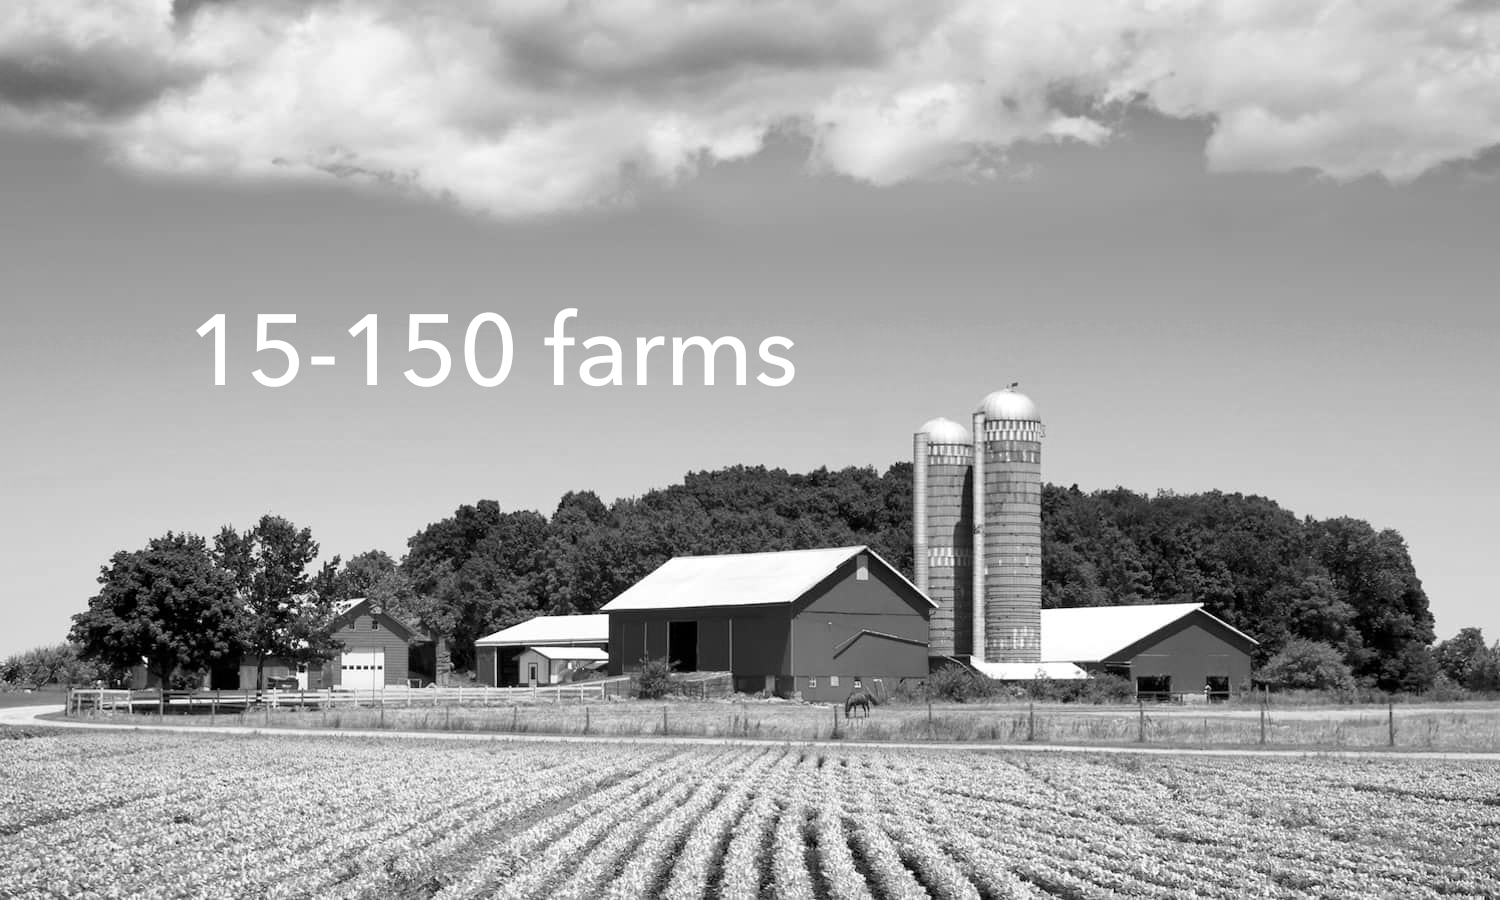
\includegraphics{../../../../crucible/farms.png}
\end{center}

\newpage

\begin{parts}
  \bonuspart[3]\hfill

    Come up with a type \code{animal} that faithfully represents the information
    of an animal on the farm. This type should have no illegal representation,
    meaning that any value of this type should represent all and only
    the relevant information to one of those specific animals.

    It should also be as un-redundant as possible, meaning there should not be
    different values that represent the same animal. It should also be as
    simple and elegant as possible.

    You may use as many \code{type} and \code{datatype} declarations as you wish.

    \begin{solutionorbox}[35em]
      \begin{codeblock}
        datatype dog_job = Pet of string | Herder | Guard

        datatype day = M | Tu | We | Th | F | Sa | Su

        type seller_info = string * real

        datatype animal_kind =
            Dog of dog_job
          | Cat
          | Horse of day * day option * string list
          | Cow of seller_info option

        type animal = string * animal_kind
      \end{codeblock}
    \end{solutionorbox}
\end{parts}


%% --- appendices --------------------------------------------------------------
%% (was \newpage

\textbf{Appendix: The \code{SEQUENCE} Signature}

\begin{codeblock}
  signature SEQUENCE =
    sig
      (* ... *)

      val empty : unit -> 'a seq
      val singleton : 'a -> 'a seq
      val tabulate : (int -> 'a ) -> int -> 'a seq
      val fromList : 'a list -> 'a seq

      val nth : 'a seq -> int -> 'a
      val null : 'a seq -> bool
      val length : 'a seq -> int
      val toList : 'a seq -> 'a list

      val filter : ('a -> bool) -> 'a seq -> 'a seq
      val map : ('a -> 'b) -> 'a seq -> 'b seq
      val reduce : ('a * 'a -> 'a) -> 'a -> 'a seq -> 'a

      (* ... *)
    end
\end{codeblock}

\vspace{20pt}

\textbf{Appendix: The \code{STREAM} Signature}

\begin{codeblock}
signature STREAM =
  sig
    (* ... *)

    val delay : (unit -> 'a front) -> 'a stream
    val expose : 'a stream -> 'a front

    val empty : 'a stream
    val cons : 'a * 'a stream -> 'a stream
    val fromList : 'a list -> 'a stream
    val tabulate : (int -> 'a) -> 'a stream

    (* ... *)
  end
\end{codeblock}



% ------------------------------------------------------------------------------

)
\newpage

\textbf{Appendix: The \code{SEQUENCE} Signature}

\begin{codeblock}
  signature SEQUENCE =
    sig
      (* ... *)

      val empty : unit -> 'a seq
      val singleton : 'a -> 'a seq
      val tabulate : (int -> 'a ) -> int -> 'a seq
      val fromList : 'a list -> 'a seq

      val nth : 'a seq -> int -> 'a
      val null : 'a seq -> bool
      val length : 'a seq -> int
      val toList : 'a seq -> 'a list

      val take : 'a seq * int -> 'a seq
      val drop : 'a seq * int -> 'a seq
      val append : 'a seq * 'a seq -> 'a seq

      val filter : ('a -> bool) -> 'a seq -> 'a seq
      val map : ('a -> 'b) -> 'a seq -> 'b seq
      val reduce : ('a * 'a -> 'a) -> 'a -> 'a seq -> 'a

      (* ... *)
    end
\end{codeblock}

\vspace{20pt}

\textbf{Appendix: The \code{STREAM} Signature}

\begin{codeblock}
signature STREAM =
  sig
    (* ... *)

    val delay : (unit -> 'a front) -> 'a stream
    val expose : 'a stream -> 'a front

    val empty : 'a stream
    val cons : 'a * 'a stream -> 'a stream
    val fromList : 'a list -> 'a stream
    val tabulate : (int -> 'a) -> 'a stream

    (* ... *)
  end
\end{codeblock}



% ------------------------------------------------------------------------------


\end{questions}

\end{document}
"
\ifdefined\blankversion
  \documentclass[addpoints,12pt]{exam}
\else
  \documentclass[addpoints,12pt,answers]{exam}
\fi

%% exam_practice.tex sets \practiceversion before reading this file; that
%% swaps every "Final Exam" below over to "Practice Final".
\ifdefined\practiceversion
  \newcommand{\examname}{Practice Final}
  \newcommand{\drawprompt}{Feel free to use this space to draw Polly the Polymorphic Parrot, the class mascot!}
  \newcommand{\drawboxheight}{1.9in}
\else
  \newcommand{\examname}{Final Exam}
  \newcommand{\drawprompt}{Feel free to use this space to draw \textbf{anything you like}. You're free!}
  \newcommand{\drawboxheight}{3.5in}
\fi

\usepackage{amsmath, amsthm, amssymb, amsfonts}
\usepackage{thmtools}
\usepackage{graphicx}
\usepackage[hidelinks]{hyperref}
\usepackage[utf8]{inputenc}
\usepackage[english]{babel}
\usepackage{framed}
\usepackage[dvipsnames]{xcolor}
\usepackage{tcolorbox}
\usepackage{tabto}
\usepackage{titling}
\usepackage{tikz}
\usepackage{dirtree}

\usetikzlibrary{patterns}
\tikzset{
level distance=13mm,
every child/.style={line width=0.3mm},
black/.style={text=white, circle, draw=black, line width=0.4mm, inner sep=4pt},
red/.style={text=white, circle, draw=black, line width=0.4mm, inner sep=4pt},
unknown/.style={text=white, circle, draw=black, line width=0.4mm, inner sep=4pt, preaction={fill, pink!90!black}, pattern=north east lines,distance=0.5pt},
}

\usepackage{changepage} % for the adjustwidth environment


\colorlet{LightGray}{White!90!Periwinkle}
\colorlet{LightOrange}{Orange!15}
\colorlet{LightGreen}{Green!15}

\newcommand{\HRule}[1]{\rule{\linewidth}{#1}}

\declaretheoremstyle[name=Theorem,]{thmsty}
\declaretheorem[style=thmsty,numberwithin=section]{theorem}
\tcolorboxenvironment{theorem}{colback=LightGray}

\declaretheoremstyle[name=Proposition,]{prosty}
\declaretheorem[style=prosty,numberlike=theorem]{proposition}
\tcolorboxenvironment{proposition}{colback=LightOrange}

\declaretheoremstyle[name=Principle,]{prcpsty}
\declaretheorem[style=prcpsty,numberlike=theorem]{principle}
\tcolorboxenvironment{principle}{colback=LightGreen}

%% This latex package provides all the utilities for
%% 15150 assignments development.
%% This package is intended to be included in writeup.tex at
%% problem level.
%% For a full list of custom commands, check 15150toolbox.md
%%
%% @author: Jolin Zhou
%% @email: jiulingz@andrew.cmu.edu

\NeedsTeXFormat{LaTeX2e}
\ProvidesPackage{toolbox-reduced}[2020/05/15 Latex toolbox for M20 Lecture Notes]

%%%%%%%%%%%%%%%%%%%%%
%% Robust Commands %%
%%%%%%%%%%%%%%%%%%%%%
% used throughout this package
\RequirePackage{etoolbox}
\RequirePackage{xparse}

% hyperlink/reference
\RequirePackage{xcolor}

% graphics
\RequirePackage{graphicx}

% emphasize
\usepackage{bm}
\DeclareTextFontCommand{\emph}{\bfseries\em}

%%%%%%%%%%%%%%%%%%%%%%%%%%%%%%%
%% Task related environments %%
%%%%%%%%%%%%%%%%%%%%%%%%%%%%%%%
% environment colors
\RequirePackage{xcolor}
\definecolor{task_color}      {RGB}{ 64, 100, 255}
\definecolor{solution_color}  {RGB}{  0,   0, 128}
\definecolor{constraint_color}{RGB}{175,   0,   0}

% task environment
\RequirePackage{framed}
\providerobustcmd{\attribute}[1]{}
\newcounter{taskcounter}
\NewDocumentEnvironment{task}{m}
{
  \stepcounter{taskcounter}
  \textbf{Task \arabic{taskcounter}.}\attribute{#1}
  \phantomsection
  \addcontentsline{toc}{subsubsection}{\textcolor{task_color}{\textbf{Task \arabic{taskcounter}.}\texorpdfstring{\attribute{#1}}{}}}
  \par
}
{
  \ifdef{\loadsolution}
    {{
      \color{solution_color}
      \begin{framed}
        \textbf{Solution \arabic{taskcounter}.}\par
        \loadsolution{#1}
      \end{framed}
    }}
    {}
  \vspace{1em}
}

% constraint environment
\newenvironment{constraint}{\color{constraint_color}\textbf{Constraint:}}{}

%%%%%%%%%%%%%%%%%%%%%%%%
%% Code Specification %%
%%%%%%%%%%%%%%%%%%%%%%%%
% spec
\RequirePackage{framed}
\usepackage{mdframed}
\newrobustcmd{\spec}[4]{
\begin{mdframed}
\code{#1 :} #2\par
\ifstrempty{#3}{}{\par REQUIRES: #3}
\ifstrempty{#4}{}{\par ENSURES: #4}
\end{mdframed}
}

%%%%%%%%%%%%%%%%%%%%%
%% Text Formatting %%
%%%%%%%%%%%%%%%%%%%%%
% symbols
\RequirePackage{amssymb, amsmath, amsthm, amsfonts}

\newrobustcmd{\stepsTo}{\Longrightarrow}
\newrobustcmd{\stepsToStar}{\Longrightarrow}
\newrobustcmd{\stepsToIn}[1]{\Longrightarrow^{#1}}

\newrobustcmd{\eeq}{\cong}

%%%%%%%%%%%%%%%%%%%%%%
%% Code Environment %%
%%%%%%%%%%%%%%%%%%%%%%
% code style
\RequirePackage{listings}
\RequirePackage{lstautogobble}
\RequirePackage{xcolor}

\newlength{\MaxSizeOfLineNumbers}%
\settowidth{\MaxSizeOfLineNumbers}{99}% Adjust to maximum number of lines
\addtolength{\MaxSizeOfLineNumbers}{.5ex}%

\newcommand{\darkBg}{8b98ad}
\definecolor{background_color}{RGB}{225, 225, 225}
\definecolor{string_color}    {RGB}{180, 156,   0}
\definecolor{keyword_color}   {RGB}{ 64, 100, 255}
\definecolor{comment_color}   {RGB}{  140, 140, 140}
\definecolor{number_color}    {RGB}{ 84,  84,  84}
\lstdefinestyle{15150code}{
    basicstyle=\ttfamily,
    numberstyle=\tiny\ttfamily\color{number_color},
    stringstyle=\color{string_color},
    keywordstyle=\color{blue!90!black},
    commentstyle=\color{comment_color},
    numbers=left,
    rulesepcolor=\color{black!20!white},
    linewidth=\textwidth,
    columns=fixed,
    tabsize=2,
    xleftmargin=\MaxSizeOfLineNumbers,
    breaklines=true,
    keepspaces=true,
    showstringspaces=false,
    captionpos=b,
    autogobble=true,
    mathescape=true,
    literate={~}{{$\thicksim$}}1
             {~=}{{$\eeq$}}1
}
\lstdefinelanguage{sml}{
    language=ML,
    morestring=[b]",
    morecomment=[s]{(*}{*)},
    morekeywords={
        bool, char, exn, int, real, string, unit, list, option,
        EQUAL, GREATER, LESS, NONE, SOME, nil,
        andalso, orelse, true, false, not,
        if, then, else, case, of, as,
        let, in, end, local, val, rec,
        datatype, type, exception, handle,
        fun, fn, op, raise, ref,
        structure, struct, signature, sig, functor,
        include, open, use, infix, infixr, o, print
    }
}

\usepackage[T1]{fontenc}

\makeatletter
\newenvironment{btHighlight}[1][]
{\begingroup\tikzset{bt@Highlight@par/.style={#1}}\begin{lrbox}{\@tempboxa}}
{\end{lrbox}\bt@HL@box[bt@Highlight@par]{\@tempboxa}\endgroup}

\newcommand\btHL[1][]{%
  \begin{btHighlight}[#1]\bgroup\aftergroup\bt@HL@endenv%
}
\def\bt@HL@endenv{%
  \end{btHighlight}%
  \egroup
}
\newcommand{\bt@HL@box}[2][]{%
  \tikz[#1]{%
    \pgfpathrectangle{\pgfpoint{1pt}{0pt}}{\pgfpoint{\wd #2}{\ht #2}}%
    \pgfusepath{use as bounding box}%
    \node[anchor=base west, fill=yellow!45,outer sep=0pt,inner xsep=1pt, inner ysep=0pt, rounded corners=3pt, minimum height=\ht\strutbox+1pt,#1]{\raisebox{1pt}{\strut}\strut\usebox{#2}};
  }%
}

\newenvironment{atHighlight}[1][]
{\begingroup\tikzset{at@Highlight@par/.style={#1}}\begin{lrbox}{\@tempboxa}}
{\end{lrbox}\at@HL@box[at@Highlight@par]{\@tempboxa}\endgroup}

\newcommand\atHL[1][]{%
  \begin{atHighlight}[#1]\bgroup\aftergroup\at@HL@endenv%
}
\def\at@HL@endenv{%
  \end{atHighlight}%
  \egroup
}
\newcommand{\at@HL@box}[2][]{%
  \tikz[#1]{%
    \pgfpathrectangle{\pgfpoint{1pt}{0pt}}{\pgfpoint{\wd #2}{\ht #2}}%
    \pgfusepath{use as bounding box}%
    \node[anchor=base west, fill=red!45,outer sep=0pt,inner xsep=1pt, inner ysep=0pt, rounded corners=3pt, minimum height=\ht\strutbox+1pt,#1]{\raisebox{1pt}{\strut}\strut\usebox{#2}};
  }%
}
\makeatother

% code inline
\newrobustcmd{\code}[2][]{{\sloppy
\ifmmode
    \text{\lstinline[language=sml,style=15150code,#1]`#2`}
\else
    {\lstinline[language=sml,style=15150code,#1]`#2`}%
\fi}}

% code block
\lstnewenvironment{codeblock}[1][]{\lstset{
  language=sml,
  style=15150code,numbers=none,#1,moredelim=**[is][\btHL]{`}{`},moredelim=**[is][\atHL]{&}{&}}}{}

% ------------------------------------------------------------------------------

\begin{document}

% Use the exam class's native headers/footers. (fancyhdr 1.11b conflicts
% with the exam class, which already defines \lhead/\rhead/\chead.)
\pagestyle{headandfoot}
\header{\examname}{}{15-150: Principles of Functional Programming}
\footer{}{\thepage}{}

% ------------------------------------------------------------------------------
% Cover Page and ToC
% ------------------------------------------------------------------------------

\setlength{\droptitle}{-8em}   % This is your set screw

\title{ \normalsize \textsc{}
		\HRule{1.5pt} \\
		\large \textbf{
      \uppercase{\examname} \\
      15-150 Principles of Functional Programming M26} \\
    \vspace{-0.15cm}
    \HRule{1.5pt}
}
\date{}

\maketitle

\vspace{-2.5cm}

Name \rule{6cm}{0.4pt} \, Andrew ID \rule{6cm}{0.4pt}

\vspace{20pt}

%% Left-aligned, and pulled slightly PAST the left margin. \noindent kills the
%% paragraph indent; the negative \hspace then moves the whole block into the
%% margin. The itemize's own \leftmargin is zeroed so the bullets themselves sit
%% at the block's edge rather than ~2.5em inside it. The old version wrapped both
%% minipages in a `center` and fought it with \hspace{-3cm}.
%% The \makebox is what keeps the negative shift from overflowing the line: it
%% pins the pair's advertised width to \textwidth and left-aligns the contents,
%% so the 0.8cm pull into the margin costs no horizontal budget.
\noindent\makebox[\textwidth][l]{%
\hspace*{-0.8cm}%
\begin{minipage}{0.585\textwidth}
\setlength{\leftmargini}{1.2em}
\begin{itemize}
  \item Write your name and Andrew ID on this page.
  \vspace{-5pt}
  \item This is a 180 minute examination of 8 parts.
  \vspace{-5pt}
  \item Answers should be short and to the point. Obey question constraints, wherever
  they appear, and write syntactically legal SML programs!
  \vspace{-5pt}
  \item At any point on this examination, you are allowed to use the \code{map},
  \code{filter}, \code{foldl}, \code{foldr}, \code{length}, \code{o}, and \code{@} functions,
  as seen in lecture.
  \vspace{-5pt}
  \item A box having lots of space does not imply the answer will be long or convoluted. If your
  answer is ugly, it's likely that something is wrong with your approach.
  \item I have full faith in you. You're going to do great.
\end{itemize}
\end{minipage}
\hspace{10pt}
\begin{minipage}{0.35\textwidth}
{\small
\vqword{}
\vpword{Max}
\begin{center}
\gradetable[v][questions]
\end{center}
}
\end{minipage}%
}

\vspace{\fill}

%% The drawing box is sized to whatever vertical room is left after the bullets
%% and the grade table. The practice exam's table has longer question titles, so
%% a fixed 2.5in box overflows and LaTeX silently drops the whole block --
%% \drawboxheight lets each version ask for a height that actually fits.
\begin{center}
  \drawprompt \\

  \vspace{8pt}

  \fbox{\rule{6in}{0pt}\rule[-0.5ex]{0pt}{\drawboxheight}}
\end{center}


\newpage

% ------------------------------------------------------------------------------

\section*{Questions}

\begin{questions}

%% --- openers -----------------------------------------------------------------
%% (drawn from the pools, so the items differ from the real final's)
\titledquestion{Types and Values}
\textbf{Types and Values}

For each expression below, give its \textbf{most general type} and value.
If the expression is not well-typed, say so and explain briefly. If it does not
evaluate to a value, say so. If it is already a value, you may write ``same''.

If the function has a recursive body that cannot be written, write "<body>" for
the function body. You should write out lambda expressions for all of the function's
arguments.

\begin{parts}
% =============================================================================
% TYPES-AND-VALUES POOL
%
% Five "most general type and value" items, each targeting a specific typing
% skill or misunderstanding rather than mechanical currying. All inferred
% types verified in SML/NJ.
%
%   1. filter with the identity as its predicate: forces 'a = bool.
%   2. Fanning one argument out to two functions: shared domain, distinct
%      codomains. Tests unification, not quantifier placement.
%   3. NWT: the [] seed and the `x + acc` body demand different accumulators.
%   4. `map` as a fold: pure inference grind, four variables in one pass. The
%      trap is collapsing the element type with the accumulator type.
%   5. foldr vs foldl with subtraction: identical types, DIFFERENT values --
%      the one item where computing the value is the whole point.
%
% Uses the same \part / solutionorlines format as the existing Types and
% Values section. Reminder that the section instructions already tell students
% to write NWT for not-well-typed and "same" for values that are already values.
% =============================================================================


% -----------------------------------------------------------------------------
% 1. filter with the identity function as its predicate.
%    Skill: a predicate must return bool, so `fn x => x` forces 'a = bool,
%    giving bool list -> bool list.
% -----------------------------------------------------------------------------
\part[2]\hfill

  \begin{codeblock}
    List.filter (fn x => x)
  \end{codeblock}

  \textbf{Type:} \begin{solutionorlines}[2em] \code{bool list -> bool list} \end{solutionorlines}

  \textbf{Value:} \begin{solutionorlines}[2em] same \end{solutionorlines}

  \vspace{10pt}


% -----------------------------------------------------------------------------
% 2. Fanning a single argument out to two functions.
%    Skill: `x` is passed to both `f` and `g`, so their DOMAINS must unify to
%    one 'a -- but their codomains are free to differ ('b and 'c). Getting
%    this right means seeing which variables are forced equal and which
%    aren't; the common error is collapsing 'b and 'c too.
% -----------------------------------------------------------------------------
\part[2]\hfill

  \begin{codeblock}
    fn (f, g) => fn x => (f x, g x)
  \end{codeblock}

  \textbf{Type:} \begin{solutionorlines}[3em] \code{('a -> 'b) * ('a -> 'c) -> 'a -> 'b * 'c} \end{solutionorlines}

  \textbf{Value:} \begin{solutionorlines}[2em] same \end{solutionorlines}

  \vspace{10pt}


% -----------------------------------------------------------------------------
% 3. NWT from the accumulator. The seed [] forces the accumulator to be a
%    list, but the body `x + acc` forces it to be an int. Same seed-vs-body
%    reasoning as item 4, so the two reinforce each other -- and unlike a
%    circularity puzzle, the conflict is a plain type mismatch a student can
%    derive. Verified in SML/NJ.
% -----------------------------------------------------------------------------
\part[2]\hfill

  \begin{codeblock}
    foldr (fn (x, acc) => x + acc) [] [1,2,3]
  \end{codeblock}

  \textbf{Type:} \begin{solutionorlines}[4em] NWT. The seed \code{[]} makes the accumulator a list, but \code{x + acc} requires \code{acc : int}. A list cannot be an \code{int}, so the two constraints conflict. (Seeding with \code{0} instead would give \code{int}.) \end{solutionorlines}

  \textbf{Value:} \begin{solutionorlines}[2em] no value \end{solutionorlines}

  \vspace{10pt}

\newpage

% -----------------------------------------------------------------------------
% 4. Pure inference grind: `map` written as a fold. Nothing tricky about the
%    rules, but four variables have to be threaded through in one pass --
%    foldr's own type, the fn's two parameters, and the [] seed.
%    The trap is collapsing the element type and the accumulator type: `x` is
%    'a and `acc` is 'b list, and they are NOT the same. A student who assumes
%    the accumulator matches the elements lands on ('a -> 'a) -> ...
%    Recognizable as `map` only AFTER the derivation. Verified in SML/NJ.
% -----------------------------------------------------------------------------
\part[2]\hfill

  \begin{codeblock}
    fn f => foldr (fn (x, acc) => f x :: acc) []
  \end{codeblock}

  \textbf{Type:} \begin{solutionorlines}[4em] \code{('a -> 'b) -> 'a list -> 'b list} \\[2pt] The seed \code{[]} and the result of \code{::} make the accumulator a \code{'b list}. Since \code{f x} is consed onto it, \code{f : 'a -> 'b} where \code{x : 'a}; \code{foldr} then takes an \code{'a list}. (This is \code{map}.) \end{solutionorlines}

  \textbf{Value:} \begin{solutionorlines}[2em] same \end{solutionorlines}

  \vspace{10pt}


% -----------------------------------------------------------------------------
% 5. foldr vs foldl with a NON-associative, non-commutative operator.
%    Skill: this is the one item where the VALUE carries the weight -- the two
%    types are identical, so the only way to distinguish them is to actually
%    unfold the recursion and see the direction. foldr gives
%    1-(2-(3-(4-0))) = ~2; foldl gives 4-(3-(2-(1-0))) = 2.
%    Verified in SML/NJ.
% -----------------------------------------------------------------------------
\part[2]\hfill

  \begin{codeblock}
    let val sub = fn (x, acc) => x - acc
    in (foldr sub 0 [1,2,3,4], foldl sub 0 [1,2,3,4]) end
  \end{codeblock}

  \textbf{Type:} \begin{solutionorlines}[2em] \code{int * int} \end{solutionorlines}

  \textbf{Value:} \begin{solutionorlines}[3em] \code{(~2, 2)}. \code{foldr} folds from the right, giving $1-(2-(3-(4-0))) = -2$. \code{foldl} folds from the left, giving $4-(3-(2-(1-0))) = 2$. \end{solutionorlines}

\end{parts}

\newpage
\titledquestion{Conceptual Questions}
\textbf{Conceptual Questions}

For each of the following, answer and \textbf{justify your answer briefly}.

\begin{parts}
%% five items, drawn from the pools (q/items/ holds them split out individually;
%% draft_*_pool.tex hold the full banks to draw from)
\part[3]\hfill

  True or false: If \code{e1} $\eeq$ \code{e2}, then \code{e1} and
  \code{e2} must have the same runtime cost.

  \begin{solutionorlines}[5em] False. Equivalence says the two expressions
  produce the same value, not that they get there the same way. For instance
  a naive \code{reverse} using \code{@} is equivalent to an accumulator-based
  one, but costs $O(n^2)$ instead of $O(n)$. \end{solutionorlines}


% -----------------------------------------------------------------------------
% 4. Mutation breaks referential transparency.
%    Misunderstanding: students believe you can always substitute equals for
%    equals (replace `f x` by its "value"), even in the presence of effects.
% -----------------------------------------------------------------------------
              %% equivalence is not runtime cost
\part[3]\hfill

  For an arbitrary \code{f : t1 -> t2} and value \code{x : t1}, for some types
  \code{t1} and \code{t2}, is it always the case that
  $$\code{f x} \;\eeq\; \code{f x}\text{?}$$

  If false, give a counterexample of SML code declaring such an \code{f} and \code{x}.

  \begin{solutionorbox}[14em]
    No. Two occurrences of the same expression are interchangeable only when
    that expression is \textbf{effect-free}. If \code{f} mutates state, each
    call can produce a different result:

    \begin{codeblock}
      val c = ref 0
      fun f () = (c := !c + 1; !c)
    \end{codeblock}

    The first \code{f ()} evaluates to \code{1} and the second to \code{2}, so
    the two are not equivalent.

    Being \textit{syntactically identical} is not enough --- equivalence is a
    claim about behavior. What mutation costs us is \textbf{referential
    transparency}: the ability to replace an expression by its value, or one
    occurrence of it by another copy, without changing what the program means.
  \end{solutionorbox}
              %% mutation breaks referential transparency
% Conceptual: let-binding is NOT the same as textual substitution under CBV.
% Two independent failure modes, both verified in SML/NJ:
%   - x unused, e1 raises:  let raises, substitution gives 5
%   - x used twice, e1 prints: let prints P once, substitution prints PP
%     (and both still return 2 -- the values agree, only the effects differ,
%      which is why "same answer" is not the same as "equivalent")
% Safe exactly when e1 is a VALUE. Also verified: x used exactly once is NOT
% sufficient (order of effects can still shift in general), so the clean
% condition to grade on is "e1 is a value" / effect-free.
\part[3]\hfill

  True or false: \code{let val x = e1 in e2 end} is equivalent to
  $[\code{e1}/x]\,\code{e2}$, the substitution of \code{e1} for all occurrences
  of \code{x} in \code{e2}. If false, give a counterexample.

  \begin{solutionorbox}[15em]
    \textbf{False.} \code{let} evaluates \code{e1} \textbf{once, up front};
    substitution instead copies the unevaluated expression to each occurrence of
    \code{x} --- so the number of times \code{e1} runs can change.

    Take \code{e1} $=$ \code{(print "P"; 1)} and \code{e2} $=$ \code{x + x}. The
    \code{let} prints \code{P} once; the substituted form
    \code{(print "P"; 1) + (print "P"; 1)} prints it \textbf{twice}. Both return
    \code{2}, so this is a case where the two agree on the value and still are
    not equivalent.

    Taking \code{e2} $=$ \code{5}, with \code{x} unused, breaks it the other
    way: for \code{e1} $=$ \code{raise Fail ""} the \code{let} raises, while the
    substituted form is just \code{5}, which evaluates fine. Here \code{let}
    runs \code{e1} once and substitution runs it \textbf{zero} times.

    The claim holds when \code{e1} is a \textbf{value} --- there is then nothing
    to evaluate, so duplicating or dropping it costs nothing. (More generally it
    suffices that \code{e1} be effect-free and terminating.)
  \end{solutionorbox}
              %% exceptions break equational reasoning
% =============================================================================
% CONCEPTUAL ITEM: what representation independence actually OBLIGES you to
% prove. Students can usually recite "the client can't tell" -- this asks for
% the shape of the argument instead: a relation, preserved by the builder, under
% which observations agree.
%
% Deliberately NOT the same punchline as mod2.tex (which asserts that two queue
% implementations are indistinguishable). Here the answer is the proof
% obligation, not the conclusion.
%
% Three operations only -- one seed, one builder, one observation -- which is
% the minimum that still forces all three clauses. Using ACC rather than SET
% also makes the two representations genuinely different TYPES (int vs
% int list), so "relation, not bijection" is immediate: every list summing to 7
% relates to the single accumulator 7.
%
% NOTE the asymmetry that students get wrong: clauses (1) and (2) are about
% R-relatedness, but clause (3) is about EQUALITY. `total` returns int, not the
% abstract t, so R does not even typecheck there.
%
% Both implementations verified to agree in SML/NJ (probe: add 10, ~7, 4).
% =============================================================================

\part[4]\hfill

  Two structures \code{A1} and \code{A2} implement the same signature
  \code{ACC}.

  \begin{codeblock}
    signature ACC =
      sig
        type t
        val init  : t
        val add   : int -> t -> t
        val total : t -> int
      end
  \end{codeblock}

  We want to show no client written against \code{ACC} can distinguish
  \code{A1} from \code{A2} --- in other words, they are equivalent through
  representation independence.

  Given a relation $R(\code{a1}, \code{a2})$ relating values \code{a1 : A1.t}
  and \code{a2 : A2.t}, write down the facts you would need to prove. Be
  careful to state each one as either an $R$-relatedness or an equivalence,
  whichever is appropriate.

  \begin{solutionorbox}[22em]
    Checking example clients cannot work --- there are infinitely many. Instead
    we show $R$ holds initially and is preserved, and that observations agree:

    \begin{enumerate}
      \item \textbf{The seeds are related:} $R(\code{A1.init}, \code{A2.init})$.

      \item \textbf{\code{add} preserves $R$.} If $R(\code{a1}, \code{a2})$,
      then for every value \code{x : int},
      $$R(\code{A1.add x a1},\; \code{A2.add x a2})$$

      \item \textbf{Observations are equal on related states.} If
      $R(\code{a1}, \code{a2})$, then
      $$\code{A1.total a1} \;\eeq\; \code{A2.total a2}$$
    \end{enumerate}

    Note the asymmetry between (2) and (3). \code{add} returns the
    \textbf{abstract} type \code{t}, so the best we can say is that its results
    are \textit{related}. But \code{total} returns \code{int}, a type the client
    can see and compare directly --- so its results must be genuinely
    \textbf{equivalent}. (Writing $R$ in (3) would not even typecheck: $R$
    relates a \code{A1.t} to a \code{A2.t}, not two \code{int}s.)

    Together these give an induction on the client's sequence of calls: the two
    structures start related, every \code{add} keeps them related, and any
    \code{total} the client performs returns the same answer either way. Since
    \code{t} is abstract, building with \code{init}/\code{add} and observing
    with \code{total} is all a client can do.
  \end{solutionorbox}

\newpage
 %% the representation-independence obligation
% Sequences: reduce is free to group the combines any way, which is what makes
% the span logarithmic. Part (i) makes them exhibit a grouping rather than just
% assert "it's parallel"; (ii) then reads the bound off their own answer.
% Associativity is only a closing remark here -- the question does not ask for
% it, so the refsol should not grade on it.
%
% Verified in SML/NJ: balanced grouping of op+ over 1..n has combine-tree depth
% exactly ceil(log2 n) -- 2 for n=4, 3 for n=8, 10 for n=1000.
% Non-associativity check: (op -) gives -10 left-nested vs 0 balanced.
\part[4]\hfill

  We are interested in the evaluation of the expression
  \code{Seq.reduce (op+) 0 S}.

  \begin{enumerate}
    \item Write an expression of \code{+} operations which is extensionally equivalent
    to the above, and represents a realistic way that it would actually be evaluated.

    \item Explain why this expression gives an advantageous performance characteristic
    to the original expression.
  \end{enumerate}

  \begin{solutionorbox}[19em]
    \textbf{(i)} A \textbf{balanced} grouping: split the sequence in half,
    reduce each half, and add the two results. On
    \code{S} $= \langle s_0, s_1, s_2, s_3 \rangle$ that is
    $$(s_0 + s_1) + (s_2 + s_3)$$
    rather than the left-nested $(((0 + s_0) + s_1) + s_2) + s_3$. Any answer
    whose parenthesization is balanced is fine --- the point is that the two
    halves appear as independent subexpressions.

    \textbf{(ii)} The two halves are independent, so they can be evaluated in
    \textbf{parallel}: the span is one $+$ plus the span of the deeper half,
    $$S(n) = S(n/2) + O(1) = O(\log n)$$
    A balanced grouping over $n$ elements is a combine tree of depth
    $\lceil \log_2 n \rceil$ --- each level halves the number of partial results
    ($n \to n/2 \to n/4 \to \cdots \to 1$) --- so only $\log n$ rounds are
    needed. The \textbf{work} is unchanged, since all $n-1$ additions still
    happen; what changes is that they no longer have to happen one after
    another. The left-nested grouping makes each addition depend on the previous
    one, a chain of depth $n$, giving span $O(n)$.

    \vspace{4pt}
    (This is also why \code{reduce} requires an \textbf{associative} combiner:
    it may pick any grouping, so all groupings must agree. \code{op+} qualifies;
    \code{op-} would not.)
  \end{solutionorbox}
             %% reduce's grouping freedom => O(log n) span
%% mod2 (two queue impls, "can a client tell?") was cut from this slot: it landed
%% on the same punchline as the modules item above it, which now asks for the
%% representation-independence proof obligation instead.
%% NOTE: draft_span_conceptual.tex (two rec calls in W => one in S?) is cut --
%% it duplicates Flattening a Tree part 4 on this same exam, and also the
%% "For any recurrence" item on the real final.
\end{parts}

%% --- proof -------------------------------------------------------------------

\newpage

\vspace*{\fill}

THIS PAGE INTENTIONALLY LEFT BLANK

I WOULDN'T LEAVE THIS BLANK UNINTENTIONALLY, THAT'S FOR SURE

WHAT DO YOU THINK I AM, STUPID?

\vspace*{\fill}

\newpage


\titledquestion{Checking Every Element}

\textbf{Checking Every Element}

For the type of polymorphic trees, consider the functions \code{treeAll}, which checks
that every element of a tree satisfies a predicate, and \code{all}, which checks
that every element of a list satisfies a predicate. Additionally provided is the
\code{inorder} function, which returns the inorder traversal of a tree.
\begin{codeblock}
  datatype 'a tree = Empty | Node of 'a tree * 'a * 'a tree

  fun treeAll p Empty = true
    | treeAll p (Node (l, x, r)) =
        p x andalso treeAll p l andalso treeAll p r

  fun all p [] = true
    | all p (x :: xs) = p x andalso all p xs

  fun inorder Empty = []
    | inorder (Node (l, x, r)) = inorder l @ (x :: inorder r)
\end{codeblock}

Checking a predicate over a tree directly should agree with flattening to the
inorder list and checking that. Prove it.

\begin{parts}
  \part[15]\hfill

    \textbf{Theorem.} For all values \code{p : 'a -> bool} and \code{T : 'a tree}:
    $$\code{treeAll p T} \;\eeq\; \code{all p (inorder T)}$$

    You may use the following facts without proof:

    \textbf{Lemma 1:} For any value
    \code{T : 'a tree}, \code{inorder T} evaluates to a value.

    \textbf{Lemma 2:} For total \code{p} and any
    value \code{L : 'a list}, \code{all p L} evaluates to a value.

    \textbf{Lemma 3:} For total \code{p} and any
    value \code{T : 'a tree}, \code{treeAll p T} evaluates to a value.

    \textbf{Lemma 4:} For total \code{p} and any
    values \code{A, B : 'a list},
    $$\code{all p (A @ B)} \;\eeq\;
      \code{all p A andalso all p B}$$

    \begin{constraint}
      You may assume \code{p} is total.
    \end{constraint}

    \begin{solutionorbox}[50em]

      By structural induction on \code{T : 'a tree}.

      \vspace{6pt}
      \textbf{Base case:} \code{T = Empty}.
      \begin{align*}
        \code{treeAll p Empty}
        &\eeq \code{true} \tag{clause 1 of \code{treeAll}} \\
        &\eeq \code{all p []} \tag{clause 1 of \code{all}} \\
        &\eeq \code{all p (inorder Empty)} \tag{clause 1 of \code{inorder}}
      \end{align*}

      \vspace{6pt}
      \textbf{Inductive case:} \code{T = Node (l, x, r).}

      \noindent IH$_l$: \code{treeAll p l} $\eeq$ \code{all p (inorder l)}.

      \noindent IH$_r$: \code{treeAll p r} $\eeq$ \code{all p (inorder r)}.

      \noindent WTS: \code{treeAll p (Node (l,x,r))} $\eeq$
      \code{all p (inorder (Node (l,x,r)))}.

      \vspace{4pt}
      We start from the \textbf{right}-hand side and reach the left:
      \begin{align*}
        & \code{all p (inorder (Node (l,x,r)))} \\
        &\eeq \code{all p (inorder l @ (x :: inorder r))}
          \tag{clause 2 of \code{inorder}} \\
        &\eeq \code{all p (inorder l)} \\
        & \quad\; \code{andalso all p (x :: inorder r)}
          \tag{Lemmas 1, 4} \\
        &\eeq \code{all p (inorder l)} \\
        & \quad\; \code{andalso (p x andalso all p (inorder r))}
          \tag{clause 2 of \code{all}} \\
        &\eeq \code{p x andalso all p (inorder l)} \\
        & \quad\; \code{andalso all p (inorder r)}
          \tag{\code{andalso} assoc.\ / comm., Lemma 2 and \code{p} total} \\
        &\eeq \code{p x andalso treeAll p l andalso treeAll p r}
          \tag{IH$_l$, IH$_r$, Lemma 3} \\
        &\eeq \code{treeAll p (Node (l,x,r))}
          \tag{clause 2 of \code{treeAll}}
      \end{align*}

      which is the left-hand side. By the principle of structural induction, the
      theorem holds for all \code{T : 'a tree}. $\qed$
    \end{solutionorbox}

    \newpage

    \begin{solutionorbox}[50em]

    \end{solutionorbox}
\end{parts}


%% --- CPS ---------------------------------------------------------------------
\newpage
\titledquestion{Filling in the Blanks}

\textbf{Filling in the Blanks}

Recall the notion of an \textit{optree}, which is a tree that corresponds to an
arithmetic expression, where the nodes are operators and the leaves are integers.

Unfortunately, a dog has eaten all of our operators!

A \textit{skeleton} is an optree whose operators are missing:

\begin{codeblock}
  datatype skel = Leaf of int | Blank of skel * skel

  datatype oper = Plus | Minus
  datatype expr = Val of int | Node of expr * oper * expr

  fun evalExpr (Val n) = n
    | evalExpr (Node (l, Plus,  r)) = evalExpr l + evalExpr r
    | evalExpr (Node (l, Minus, r)) = evalExpr l - evalExpr r
\end{codeblock}

Our goal will be to take a \code{skel} and fill in each \code{Blank} node to obtain
an \code{expr}. Each \code{Blank} may become either \code{Plus} or \code{Minus},
so a skeleton with $k$ blanks has $2^k$ fillings:

\begin{center}
\begin{tikzpicture}[
  level 1/.style={sibling distance=15mm},
  level 2/.style={sibling distance=10mm},
  level distance=10mm,
  every node/.style={inner sep=1.5pt},
  blank/.style={circle, draw, dashed, minimum size=6mm},
  op/.style={circle, draw, fill=LightGreen, minimum size=6mm},
  lf/.style={rectangle, draw, minimum size=5.5mm},
  treecap/.style={anchor=north},          % captions share one baseline
]
%% Each tree is rooted at y=0 and is 2 levels deep, so every caption
%% hangs from the same y -- keeps the three columns visually aligned.
\def\capy{-2.55}

%% ---- skeleton ----
\begin{scope}
  \node[blank] {?}
    child {node[blank] {?}
      child {node[lf] {5}}
      child {node[lf] {3}}}
    child {node[lf] {2}};
  \node[treecap] at (0,\capy) {\small skeleton};
\end{scope}

\node at (2.35,-1.0) {\large $\rightsquigarrow$};

%% ---- filling A ----
\begin{scope}[xshift=4.2cm]
  \node[op] {$+$}
    child {node[op] {$-$}
      child {node[lf] {5}}
      child {node[lf] {3}}}
    child {node[lf] {2}};
  \node[treecap] at (0,\capy) {\small $(5-3)+2 = 4$};
\end{scope}

%% ---- filling B ----
\begin{scope}[xshift=8.0cm]
  \node[op] {$+$}
    child {node[op] {$+$}
      child {node[lf] {5}}
      child {node[lf] {3}}}
    child {node[lf] {2}};
  \node[treecap] at (0,\capy) {\small $(5+3)+2 = 10$};
\end{scope}
\end{tikzpicture}
\end{center}

\noindent
This skeleton has four fillings in all, evaluating to \code{4}, \code{10},
\code{0}, and \code{6}. Nothing fills it to \code{7}.

We search for a filling in CPS. One continuation \code{k} is offered each candidate, and returns
\code{SOME} to accept it or \code{NONE} to make \code{fill} try the next.

\begin{parts}
  \part[12]\hfill

    Implement \code{fill}:

    \spec
      {fill}
      {\code{skel -> (expr * int -> expr option) -> expr option}}
      {\code{k} is total}
      {\code{fill s k} offers \code{k} each way of filling \code{s}, as a pair
      \code{(e, v)} of a filled-in expression \code{e} and its value \code{v}.
      It returns the first \code{SOME} that \code{k} produces, or \code{NONE} if
      \code{k} rejects every filling.}

    \begin{solutionorbox}[26em]
      \begin{codeblock}
        fun fill (Leaf n) k = k (Val n, n)
          | fill (Blank (l, r)) k =
              fill l (fn (le, a) =>
                fill r (fn (re, b) =>
                  case k (Node (le, Plus, re), a + b) of
                    SOME res => SOME res
                  | NONE => k (Node (le, Minus, re), a - b)))
      \end{codeblock}

      To fill a \code{Blank}, we fill the left subtree; its continuation fills the
      right subtree; and \textit{that} continuation has both filled subtrees
      \code{le} and \code{re} in hand, so it can build the node. It offers the
      \code{Plus} version to \code{k}; only if \code{k} rejects it (\code{NONE})
      does it fall back to the \code{Minus} version.
    \end{solutionorbox}

  \part[3]\hfill

    Using \code{fill}, implement \code{solve}.

    \spec
      {solve}
      {\code{skel -> int -> expr option}}
      {\code{true}}
      {\code{solve s target} evaluates to \code{SOME e}, where \code{e} is a
      filling of \code{s} with \code{evalExpr e} $\eeq$ \code{target}, or
      \code{NONE} if no such filling exists.}

    \begin{solutionorbox}[12em]
      \begin{codeblock}
        fun solve s target =
          fill s (fn (e, v) =>
            if v = target then SOME e else NONE)
      \end{codeblock}

      The continuation is the goal test: accept a candidate (\code{SOME e}) when
      its value matches the target, and reject it (\code{NONE}) otherwise ---
      which tells \code{fill} to keep searching.
    \end{solutionorbox}

  \newpage

  \part[8]\hfill

    \code{fill} stops at the first accepted filling. Now we want all of them.
    Implement \code{fillAll}:

    \spec
      {fillAll}
      {\code{skel -> (expr * int -> 'a list) -> 'a list}}
      {\code{k} is total}
      {\code{fillAll s k} evaluates to the concatenation of \code{k (e, v)} over
      \textbf{every} filling \code{(e, v)} of \code{s}.}

    Then implement \code{solveAll} using it:

    \spec
      {solveAll}
      {\code{skel -> int -> expr list}}
      {\code{true}}
      {\code{solveAll s target} evaluates to a list of all fillings \code{e} of
      \code{s} with \code{evalExpr e} $\eeq$ \code{target}.}

    \begin{solutionorbox}[30em]
      \begin{codeblock}
        fun fillAll (Leaf n) k = k (Val n, n)
          | fillAll (Blank (l, r)) k =
              fillAll l (fn (le, a) =>
                fillAll r (fn (re, b) =>
                    k (Node (le, Plus,  re), a + b)
                  @ k (Node (le, Minus, re), a - b)))

        fun solveAll s target =
          fillAll s (fn (e, v) =>
            if v = target then [e] else [])
      \end{codeblock}

      The only change from \code{fill} is what happens at a \code{Blank}: instead
      of trying \code{Plus} and falling back to \code{Minus} only on rejection,
      we take \textbf{both} and \code{@} their results together --- so nothing is
      ever cut off. The continuation reports zero or more results per candidate
      (\code{[e]} to keep it, \code{[]} to drop it), and the concatenation
      accumulates them all.
    \end{solutionorbox}
\end{parts}


%% --- streams -----------------------------------------------------------------
\newpage
\titledquestion{The Fringe of the Matter}

\textbf{The Fringe of the Matter}

Consider shrubs, which store data only at their leaves:
\begin{codeblock}
  datatype 'a shrub = Leaf of 'a | Branch of 'a shrub * 'a shrub
\end{codeblock}

The \textbf{fringe} of a shrub is the sequence of its leaf values, read from left
to right. For instance, both of the following trees have fringe
\code{1, 2, 3}, even though they have completely different shapes:

\begin{center}
  \begin{tikzpicture}[
    level distance=10mm,
    level 1/.style={sibling distance=20mm},
    level 2/.style={sibling distance=11mm},
    every node/.style={font=\small},
    dot/.style={circle, fill, inner sep=1.5pt}
  ]
    \node[dot] {}
      child{node[dot] {}
        child{node {\code{1}}}
        child{node {\code{2}}}
      }
      child{node {\code{3}}}
    ;
  \end{tikzpicture}
  \hspace{2cm}
  \begin{tikzpicture}[
    level distance=10mm,
    level 1/.style={sibling distance=20mm},
    level 2/.style={sibling distance=11mm},
    every node/.style={font=\small},
    dot/.style={circle, fill, inner sep=1.5pt}
  ]
    \node[dot] {}
      child{node {\code{1}}}
      child{node[dot] {}
        child{node {\code{2}}}
        child{node {\code{3}}}
      }
    ;
  \end{tikzpicture}
\end{center}

We are curious whether two shrubs have the same fringe. We will choose to
model the fringe of a shrub as a \textbf{stream} of its leaf values, avoiding
constructing the list of all the leaf values up front. We write
\code{S} to refer to the \code{STREAM} library, whose signature is in the appendix.

You are given \code{append : 'a stream -> 'a stream -> 'a stream}, which appends two streams,
as a helper function.

\begin{parts}
  \part[5]\hfill

    Using \code{append}, implement \code{fringe}.

    \spec
      {fringe}
      {\code{'a shrub -> 'a S.stream}}
      {\code{true}}
      {\code{fringe T} evaluates to the stream of the leaf values of \code{T},
      in left-to-right order.}

    \begin{solutionorbox}[14em]
      \begin{codeblock}
        fun fringe (Leaf x) = S.cons (x, S.empty)
          | fringe (Branch (L, R)) = append (fringe L) (fringe R)
      \end{codeblock}

      The stream's suspended tail is what lets us stop early: the leaves of the
      right subtree are not produced until something actually asks for them.
    \end{solutionorbox}

  \newpage

  \part[3]\hfill

    Suppose we had the following bad implementation of \code{append}:
    \begin{codeblock}
      fun appendBad S1 S2 =
        case S.expose S1 of
          S.Empty => S2
        | S.Cons (x, S1') => S.cons (x, appendBad S1' S2)
    \end{codeblock}

    Is \code{appendBad} maximally lazy? If not, what goes wrong, and why does it
    matter here?

    \begin{solutionorbox}[10em]
      No. It calls \code{S.expose S1} \textbf{before} anyone has requested an
      element of the result, forcing a step of \code{S1}'s computation
      immediately --- so merely \textit{building} the appended stream already
      does work. The \code{S.delay} in the given version prevents this: nothing
      is exposed until the resulting stream is itself exposed.

      This matters here because \code{fringe} appends a stream per
      \code{Branch}. With \code{appendBad}, simply constructing
      \code{fringe T} would force its way down the shrub eagerly, and
      \code{sameFringe} (below) could no longer short-circuit --- it would end up
      producing the fringes it was supposed to avoid building.
    \end{solutionorbox}

  \part[8]\hfill

    Implement \code{sameFringe}. You may find it helpful to define a helper function.

    \spec
      {sameFringe}
      {\code{'a shrub * 'a shrub -> bool}}
      {\code{true}}
      {\code{sameFringe (T1, T2)} $\eeq$ \code{true} if \code{T1} and \code{T2}
      have the same fringe, and \code{false} otherwise.}

    \begin{constraint}
      Your solution must stop on the first mismatched leaf.
    \end{constraint}

    \vspace{3.5cm}

    THIS SECTION LEFT BLANK -- WRITE ANSWER ON NEXT PAGE

    \newpage



    \begin{solutionorbox}[30em]
      \begin{codeblock}
        fun sameFringe (T1, T2) =
          let
            fun walk S1 S2 =
              case (S.expose S1, S.expose S2) of
                (S.Empty, S.Empty) => true
              | (S.Cons (x, S1'), S.Cons (y, S2')) =>
                  x = y andalso walk S1' S2'
              | _ => false
          in
            walk (fringe T1) (fringe T2)
          end
      \end{codeblock}

      The \code{andalso} is what short-circuits: on the first mismatched pair of
      leaves, \code{walk} returns \code{false} without exposing any more of
      either stream. The final \code{\_} case handles fringes of different
      lengths (one stream empty while the other is not).
    \end{solutionorbox}

  \part[3]\hfill

    Why can this be more efficient than flattening both shrubs to lists and
    comparing with \code{=}?

    \begin{solutionorbox}[10em]
      The list-based approach must fully traverse \textbf{both} trees and build
      \textbf{both} complete fringe lists before it can compare anything. The
      stream-based approach produces leaves only on demand and compares them one
      at a time, so as soon as the two fringes first differ it stops --- having
      traversed only as far into each shrub as that first mismatch, and never
      allocating either full fringe.
    \end{solutionorbox}
\end{parts}


%% --- folding -----------------------------------------------------------------
\newpage
\titledquestion{Two Accumulators}

\textbf{Two Accumulators}

\code{foldl} threads one accumulator through a list. Some computations want
\textbf{two}, each able to depend on the other. We will build \code{fold2},
which threads two, and then use it.

\begin{parts}
  \part[8]\hfill

    Implement \code{fold2}:

    \spec
      {fold2}
      {\code{('a * 'b * 'c -> 'b * 'c) -> 'b * 'c -> 'a list -> 'b * 'c}}
      {\code{g} is total}
      {\code{fold2 g (b0, c0) [x1, ..., xn]} threads the two accumulators
      left-to-right: starting from \code{(b0, c0)}, each element \code{xi}
      updates the accumulators by \code{g (xi, b, c)}. It evaluates to the
      final pair of accumulators.}

    That is: like \code{foldl}, except \code{g} receives both accumulators and
    produces both, so either may depend on the other.

    \begin{solutionorbox}[16em]
      \begin{codeblock}
        fun fold2 g (b, c) [] = (b, c)
          | fold2 g (b, c) (x::xs) =
              let
                val (b', c') = g (x, b, c)
              in
                fold2 g (b', c') xs
              end
      \end{codeblock}
    \end{solutionorbox}

  \newpage

  \part[8]\hfill

    The \textit{best prefix sum} is the largest running prefix sum, counting the
    empty prefix as \code{0}. For \code{[3, ~2, ~2, 5]} the prefix sums are
    \code{3, 1, ~1, 4}, so the answer is \code{4}. Implement \code{bestPrefix}:

    \spec
      {bestPrefix}
      {\code{int list -> int}}
      {\code{true}}
      {\code{bestPrefix xs} evaluates to the largest running prefix sum of
      \code{xs}, or \code{0} if every prefix sum is negative.}

    \begin{constraint}
      You must use \code{fold2}, and traverse the list only once. You may not
      use explicit recursion.
    \end{constraint}

    \begin{solutionorbox}[18em]
      The two accumulators are the running \textbf{sum} of the prefix so far,
      and the \textbf{best} prefix sum seen so far. The best cannot be updated
      without the running sum --- that is the interaction.

      \begin{codeblock}
        fun bestPrefix xs =
          #2 (fold2
                (fn (x, sum, best) =>
                   let
                     val sum' = sum + x
                   in
                     (sum', Int.max (best, sum'))
                   end)
                (0, 0)
                xs)
      \end{codeblock}

      We start both accumulators at \code{0} (the empty prefix has sum \code{0},
      and it is a candidate for the best). At each element we advance the sum,
      then take the max of the old best and the \textit{new} sum. The answer is
      the second accumulator.
    \end{solutionorbox}

  \newpage

  \part[4]\hfill

    A student claims \code{fold2} is strictly more powerful than \code{foldl}.
    Settle it by implementing \code{foldl} in terms of \code{fold2}, to show \code{fold2}
    is at least as powerful.

    \begin{solutionorbox}[20em]
      \code{foldl} is the special case of \code{fold2} that ignores the second
      accumulator (we thread \code{unit} through it):

      \begin{codeblock}
        fun foldl' f z xs =
          #1 (fold2 (fn (x, acc, u) => (f (x, acc), u)) (z, ()) xs)
      \end{codeblock}
    \end{solutionorbox}
\end{parts}


%% --- work/span ---------------------------------------------------------------
\newpage
\titledquestion{Flattening a Tree}

\textbf{Flattening a Tree}

Here are two versions of \code{fringe}, which flattens a shrub to the list of its
leaves:
\begin{codeblock}
  datatype 'a shrub = Leaf of 'a | Branch of 'a shrub * 'a shrub

  (* A *)
  fun fringe (Leaf x)      = [x]
    | fringe (Branch (l, r)) = fringe l @ fringe r

  (* B *)
  fun fringeAcc (Leaf x) acc      = x :: acc
    | fringeAcc (Branch (l, r)) acc = fringeAcc l (fringeAcc r acc)
  fun fringe' t = fringeAcc t []
\end{codeblock}

Both produce the same list. Assume the shrub is \textbf{complete} of depth
\code{d}, so it has $n = 2^d$ leaves. You may use that \code{A @ B} has work and
span $O(length A)$.

\begin{parts}
  \part[4]\hfill

    Write and solve the \textbf{work} recurrence for version A, in terms of the
    number of leaves \code{n}.

    \begin{solutionorbox}[20em]
      Each recursive call handles $n/2$ leaves, and the append copies the left
      result, which has $n/2$ elements:
      $$W(n) = 2W(n/2) + O(n).$$
      By the recursion tree each of the $\log n$ levels does $O(n)$ work, so
      $$W(n) = O(n \log n).$$
    \end{solutionorbox}

  \newpage

  \part[4]\hfill

    Now give the same cost \textbf{in terms of the depth} \code{d}, both as a
    recurrence and solved.

    \begin{solutionorbox}[25em]
      A shrub of depth \code{d} has two subtrees of depth $d-1$, and the append
      copies $2^{d-1}$ elements:
      $$W(d) = 2W(d-1) + O(2^d) = O(d \cdot 2^d).$$

      This is the same bound: substituting $n = 2^d$ (so $d = \log n$) into
      $O(d \cdot 2^d)$ gives $O(n \log n)$.
    \end{solutionorbox}

  \part[2]\hfill

    Write the \textbf{work} recurrence for version B, in terms of the number of
    leaves \code{n}. You do not need to solve it.

    \begin{solutionorbox}[15em]
      Each leaf is consed on exactly once and no list is copied, so the only
      cost outside the recursive calls is constant:
      $$W(n) = 2W(n/2) + O(1)$$
    \end{solutionorbox}

  \newpage

  \part[3]\hfill

    Write the \textbf{span} recurrence for each version, in terms of the number of
    leaves \code{n}. You do not need to solve it.

    \begin{solutionorbox}[20em]
      \textbf{A:} the two recursive calls do not use each other's results, so
      they run in parallel and only the deeper one counts; the append combining
      them is sequential and costs $O(n)$:
      $$S(n) = S(n/2) + O(n)$$

      \textbf{B:} in \code{fringeAcc l (fringeAcc r acc)} the outer call takes
      the inner call's result as an argument, so the two calls are
      \textbf{dependent} and both appear in the recurrence:
      $$S(n) = 2S(n/2) + O(1)$$

      The contrast to notice is the coefficient: A's recursive calls are
      independent (one $S(n/2)$), while B's accumulator threading serialises
      them (two).
    \end{solutionorbox}
\end{parts}

\newpage


%% --- imperative --------------------------------------------------------------
\titledquestion{Arrays}

\textbf{Arrays}

We discussed \textit{sequences} in lecture, which are immutable arrays that
admit nice parallel properties due to having constant-time access to each
index.

Sequences, however, have some memory disadvantages. For instance, to map a function
on a sequence, we need to allocate a brand new sequence. For some applications,
this can be rather disadvantageous.

Imperative arrays can perform \textit{in-place} operations, which means performing
operations on an array \textit{without} having to allocate a brand new array. In
other words, by reusing the same space in place, via mutation.

Sequences are not naturally in-place. But what if we combine them with reference
cells? Consider the following type:

\begin{codeblock}
  type 'a array = 'a ref Seq.t
\end{codeblock}

Now we have recovered arrays from sequences.

\begin{parts}
  \part[5]\hfill

    Implement the following function:
    \spec
      {update}
      {\code{'a array -> int * 'a -> unit}}
      {\code{true}}
      {\code{update A (i, x)} updates the \code{i}th index of the array \code{A} to
      the element \code{x}. Raises \code{Range} if out of range.}

    Assume that there exists an exception \code{Range} declared somewhere.

    \begin{solutionorbox}[15em]
      \begin{codeblock}
        fun update A (n, x) =
          if n >= Seq.length x orelse n < 0 then
            raise Range
          else
            Seq.nth A n := x
      \end{codeblock}
    \end{solutionorbox}

  \newpage

  \part[5]\hfill

    Implement the following function:
    \spec
      {tabulate}
      {\code{(int -> 'a) -> int -> 'a array}}
      {\code{f} is total, \code{n >= 0}}
      {\code{tabulate f n} evaluates to a fresh array of length \code{n},
      where the \code{i}th index is equivalent to \code{f i}}

    \begin{solutionorbox}[15em]
      \begin{codeblock}
        fun tabulate f n =
          Seq.tabulate (fn i => ref (f i)) n
      \end{codeblock}
    \end{solutionorbox}

  \part[5]\hfill

    Implement the following function:
    \spec
      {map}
      {\code{('a -> 'a) -> 'a array -> unit}}
      {\code{f} is total}
      {\code{map f A} maps all the elements \code{x} in \code{A} to \code{f x},
      in-place}

    You may assume the existence of
    \code{Seq.iter : ('a -> unit) -> 'a Seq.t -> unit}, which simply
    applies a function to each element of a sequence.

    \begin{solutionorbox}[15em]
      \begin{codeblock}
        fun map f A =
          (Seq.map (fn r => r := f (!r)) A; ())
      \end{codeblock}
    \end{solutionorbox}

  \newpage

  \part[12]\hfill

    Now, let's do a fun use case for in-place algorithms: in-place sorting.\footnote{
      Any reasonable $O(n \log n)$ algorithm would be absurd to ask you to implement
      during an exam, especially in-place. But we can do a basic one. Let's do bubblesort.
    }

    Bubblesort is a sorting algorithm which is done by repeatedly swapping
    out-of-order adjacent elements, until the array is completely sorted. We can
    describe the algorithm as follows:

    \begin{lstlisting}[style=15150code, numbers=none]
      for adjacent pairs in array:
        if pair is out of order:
          swap them

      if any pairs were swapped, go back to loop
    \end{lstlisting}

    Implement the following function:
    \spec
      {bubsort}
      {\code{('a * 'a -> order) -> 'a array -> unit}}
      {\code{cmp} is a valid comparison function}
      {\code{bubsort cmp A} sorts the array \code{A} via \code{cmp}, in-place}

    You may use the following \code{swap : 'a ref -> 'a ref -> unit} function:

    \begin{codeblock}
      fun swap r1 r2 =
        let
          val r1_v = !r1
        in
          ( r1 := !r2; r2 := r1_v )
        end
    \end{codeblock}

    We give you the following skeleton of code, where
    \code{adj_pairs : 'a array -> ('a ref * 'a ref) list} obtains all of the
    adjacent pairs within a list. So for instance,
    \code{adj_pairs} $\langle \code{r1}, \code{r2}, \code{r3} \rangle$ $\eeq$
    \code{[(r1, r2), (r2, r3)]}.

    \begin{codeblock}
      fun bubsort cmp A =
        let
          val pairs = adj_pairs A

          fun aux pairs = (* Implement me! *)
        in
          aux pairs
        end
    \end{codeblock}

    \newpage

    \begin{solutionorbox}[45em]
      \begin{codeblock}
        fun aux pairs =
          if
            List.foldl (fn ((r1, r2), acc) =>
              case cmp (!r1, !r2) of
                GREATER => (swap r1 r2; true)
              | _ => acc
            ) false pairs
          then
            aux pairs
          else
            ()
      \end{codeblock}

    \end{solutionorbox}
\end{parts}

\newpage


%% --- appendices --------------------------------------------------------------
\newpage

\textbf{Appendix: The \code{SEQUENCE} Signature}

\begin{codeblock}
  signature SEQUENCE =
    sig
      (* ... *)

      val empty : unit -> 'a seq
      val singleton : 'a -> 'a seq
      val tabulate : (int -> 'a ) -> int -> 'a seq
      val fromList : 'a list -> 'a seq

      val nth : 'a seq -> int -> 'a
      val null : 'a seq -> bool
      val length : 'a seq -> int
      val toList : 'a seq -> 'a list

      val filter : ('a -> bool) -> 'a seq -> 'a seq
      val map : ('a -> 'b) -> 'a seq -> 'b seq
      val reduce : ('a * 'a -> 'a) -> 'a -> 'a seq -> 'a

      (* ... *)
    end
\end{codeblock}

\vspace{20pt}

\textbf{Appendix: The \code{STREAM} Signature}

\begin{codeblock}
signature STREAM =
  sig
    (* ... *)

    val delay : (unit -> 'a front) -> 'a stream
    val expose : 'a stream -> 'a front

    val empty : 'a stream
    val cons : 'a * 'a stream -> 'a stream
    val fromList : 'a list -> 'a stream
    val tabulate : (int -> 'a) -> 'a stream

    (* ... *)
  end
\end{codeblock}



% ------------------------------------------------------------------------------



\end{questions}

\end{document}
